% RECOMB 2027 draft manuscript.
% Expanded from planning scaffold using outline.md and main.tex.
% Official CFP checked 2026-10-29: Letter, >=10pt, 1in margins, <=10 main pages.
\documentclass[10pt,letterpaper]{article}
\usepackage[margin=1in]{geometry}
\usepackage[T1]{fontenc}
\usepackage[utf8]{inputenc}
\usepackage{lmodern}
\usepackage{amsmath,amssymb}
\usepackage{graphicx,booktabs}
\graphicspath{{../figures/}}
\usepackage{tabularx}
\usepackage{caption}
\captionsetup{font=normalsize,skip=4pt}
\usepackage{float}
\usepackage[skins,breakable]{tcolorbox}
\usepackage[hidelinks]{hyperref}
\usepackage{cite}

% Let full-size figures share pages with text while keeping the required margins.
\renewcommand{\topfraction}{0.95}
\renewcommand{\bottomfraction}{0.95}
\renewcommand{\textfraction}{0.05}
\renewcommand{\floatpagefraction}{0.8}
\setcounter{topnumber}{3}
\setcounter{bottomnumber}{3}
\setcounter{totalnumber}{6}
\setlength{\textfloatsep}{10pt plus 2pt minus 2pt}
\setlength{\floatsep}{8pt plus 2pt minus 2pt}
\setlength{\intextsep}{10pt plus 2pt minus 2pt}
\setlength{\emergencystretch}{1em}

% Keep abstract text and author footnotes at the 10 pt submission minimum.
\makeatletter
\renewcommand\small{\@setfontsize\small{10}{12}}
\renewcommand\footnotesize{\@setfontsize\footnotesize{10}{12}}
\makeatother

\newtcolorbox{promptbox}[1]{%
  enhanced,
  breakable,
  colback=black!2,
  colframe=black!60,
  boxrule=0.65pt,
  arc=1.4pt,
  left=8pt,
  right=8pt,
  top=5pt,
  bottom=6pt,
  title={#1},
  fonttitle=\bfseries\normalsize,
  coltitle=black,
  colbacktitle=black!8,
  before upper={\normalsize\setlength{\parskip}{0.35em}},
}
\newenvironment{promptitems}{%
  \begin{itemize}%
    \setlength{\itemsep}{0.15em}%
    \setlength{\parsep}{0pt}%
    \setlength{\topsep}{0.25em}%
    \setlength{\leftmargin}{1.2em}%
}{\end{itemize}}
\newcommand{\prompthead}[1]{\par\smallskip\noindent\textbf{#1}\par}

\title{MicroBioAgent: Closed-Loop Planning and Asynchronous Execution for
Autonomous Microbiome Analysis}
\author{Zeming Li\thanks{Email: \url{cszmli@comp.hkbu.edu.hk}} \and Jingjing
Wang \and Chonghao Wang \and Yi Ding \and Lu Zhang\thanks{Corresponding author.
Email: \url{ericluzhang@hkbu.edu.hk}}}
\date{Department of Computer Science, Hong Kong Baptist University\\Hong Kong
SAR 999077, China}

\begin{document}
\begin{titlepage}
\maketitle
\begin{abstract}
    Microbiome data analysis demands customized workflows tailored to specific
    biological questions, sequencing modalities, and data properties.  However,
    constructing and executing these workflows requires navigating heterogeneous
    software dependencies, reference databases, and multi-step parameter tuning.
    Here, we present MicroBioAgent, an autonomous, domain-specific agent
    framework
    that translates high-level biological queries into executable,
    study-specific
    pipelines across 16S rRNA amplicon, reference-based shotgun, and de novo
    assembly-based metagenomics.  Rather than relying on static pipeline
    templates,
    MicroBioAgent employs a closed-loop execution architecture: it dynamically
    selects and runs bioinformatics tools within user-controlled environments
    while
    iteratively inspecting intermediate outputs to adapt downstream analytical
    decisions.  Furthermore, to address the long-running nature of metagenomic
    computation, we introduce an asynchronous background task-management
    mechanism
    that reduces large language model (LLM) token consumption by over 50\%
    while enabling real-time plan
    adjustment and automated workflow resumption.  We systematically evaluated
    MicroBioAgent across three benchmarks of increasing complexity: (1)~paired
    amplicon and shotgun profiling of tomato rhizosphere microbiomes,
    (2)~taxonomic
    and functional profiling coupled with machine-learning classification in a
    colorectal cancer cohort, and (3)~de novo metagenomic assembly,
    metagenome-assembled genome (MAG) binning, and metabolic pathway
    reconstruction
    in a polyethylene degradation study.  Across all benchmarks, MicroBioAgent
    faithfully recapitulated the primary biological findings of the original
    studies, exhibiting high analytical concordance despite expected tool- and
    database-dependent variations.  In systematic robustness evaluations across
    27
    independent runs spanning three backbone LLMs and three
    prompt-complexity tiers, MicroBioAgent achieved a 98.8\% task completion
    rate
    and yielded highly reproducible diversity and differential-abundance
    estimates.
    MicroBioAgent establishes a scalable, adaptive paradigm for end-to-end
    computational microbiome research.
\end{abstract}
\vfill
\noindent\textbf{Keywords:} microbiome analysis, 16S rRNA, shotgun
metagenomics, MAGs, AI agent, asynchronous execution
\end{titlepage}
\setcounter{page}{1}

\section{Introduction}

Microbiome studies connect sequencing-data processing with taxonomic and
functional characterization and downstream statistics, requiring researchers to
select tools and configure software and reference
resources~\cite{knight2018bestpractices}. Advances in high-throughput
sequencing have enabled comprehensive profiling of microbial communities across
plant, human, and environmental ecosystems. However, converting raw sequencing
reads into reliable scientific findings demands multi-stage analytical
workflows. Researchers must select appropriate computational algorithms,
maintain complex software dependencies across isolated package environments,
configure massive reference databases, write custom post-processing scripts,
and execute downstream statistical tests. These multifaceted technical and
bioinformatic hurdles present substantial barriers for life scientists without
specialized computational training, often limiting their ability to explore
alternate analytical strategies or conduct customized investigations
independently~\cite{tong2020genepiper,liu2021practical}.

To automate complex analytical pipelines, computational workflow managers and
general biomedical AI agents have emerged as two key paradigms. Computational
workflow systems such as Snakemake and Nextflow offer reproducible, scalable
dependency tracking and parallel
execution~\cite{koster2012snakemake,ditommaso2017nextflow}. Nevertheless, these
engines require explicit, predefined execution graphs and pipeline
specifications; researchers must still determine which analyses to run,
manually structure workflow scripts, and interpret intermediate findings.
Concurrently, LLM agents have demonstrated substantial promise in general
biomedical problem solving and automated code execution, as seen in AutoBA,
Biomni, BioMedAgent, BioMaster, and
M3A~\cite{zhou2024autoba,huang2026biomni,bu2026biomedagent,su2026biomaster,johri2026m3a}.

In the microbiome domain, MetaClaw recently introduced an agent framework that
bridges predefined cloud-based upstream workflows (hosted on FlowHub) with
customizable local downstream skills~\cite{zhang2026metaclaw}. However, this
architecture presents two key limitations in practical research. First, relying
on external cloud platforms restricts analyses subject to data privacy
regulations, transfer bandwidth constraints, or institutional policies that
require raw sequencing reads to remain on local infrastructure. Second,
MetaClaw monitors long-running computations through repeated polling within the
active conversation. For metagenomic tasks requiring hours of processing,
continuous status checks rapidly consume conversational context, incur
unnecessary token overhead, and prevent researchers from providing feedback or
adjusting downstream plans while computations are underway.

To address these challenges, we present MicroBioAgent, a domain-specific agent
framework for end-to-end computational microbiome research. MicroBioAgent
translates high-level biological objectives into executable analyses without
relying on static workflow templates. By pairing modular domain skills with
local software environments and reference registries, the agent dynamically
selects tools, adjusts parameters, and inspects intermediate outputs to guide
downstream steps. To manage compute-intensive workflows efficiently, we
introduce an background task coordination mechanism. This
mechanism decouples long-running shell execution from the conversational
dialogue, eliminating polling overhead while enabling researchers to
interactively refine pending analyses before automated workflow resumption.

We systematically evaluate MicroBioAgent across 230 sequencing libraries from
three published datasets covering paired amplicon and shotgun profiling,
functional metagenomic classification, and long-read genome reconstruction.
Across all benchmarks, MicroBioAgent accurately executed the required
analytical pipelines and recapitulated the biological findings of the original
studies. In addition, systematic robustness evaluations across 27 independent
sessions demonstrated high task completion rates and reproducible quantitative
outputs, while ablation experiments confirmed that our asynchronous
coordination mechanism reduces token consumption by over 50\% compared to
standard polling baselines.

\section{Methods}

MicroBioAgent is an autonomous conversational agent designed for end-to-end
computational microbiome research, implemented on the open-source OpenClaw
runtime (Figure~\ref{fig:architecture}). The framework coordinates three core
functional components: (1)~a modular library of domain-specific skills paired
with host runtime and reference registries; (2)~a closed-loop execution engine
that dynamically plans, executes, and validates multi-step analyses on local
infrastructure; and (3)~an task management mechanism that
decouples long-running bioinformatics computations from the conversational
dialogue. By executing shell commands and custom scripts directly on the host
system, MicroBioAgent eliminates dependencies on external cloud platforms or
rigid, hardcoded pipeline templates. Implementation details and software/database
versions are provided in Appendix~\ref{app:implementation} and
Table~\ref{tab:software-versions}.

\begin{figure}[t]
\centering
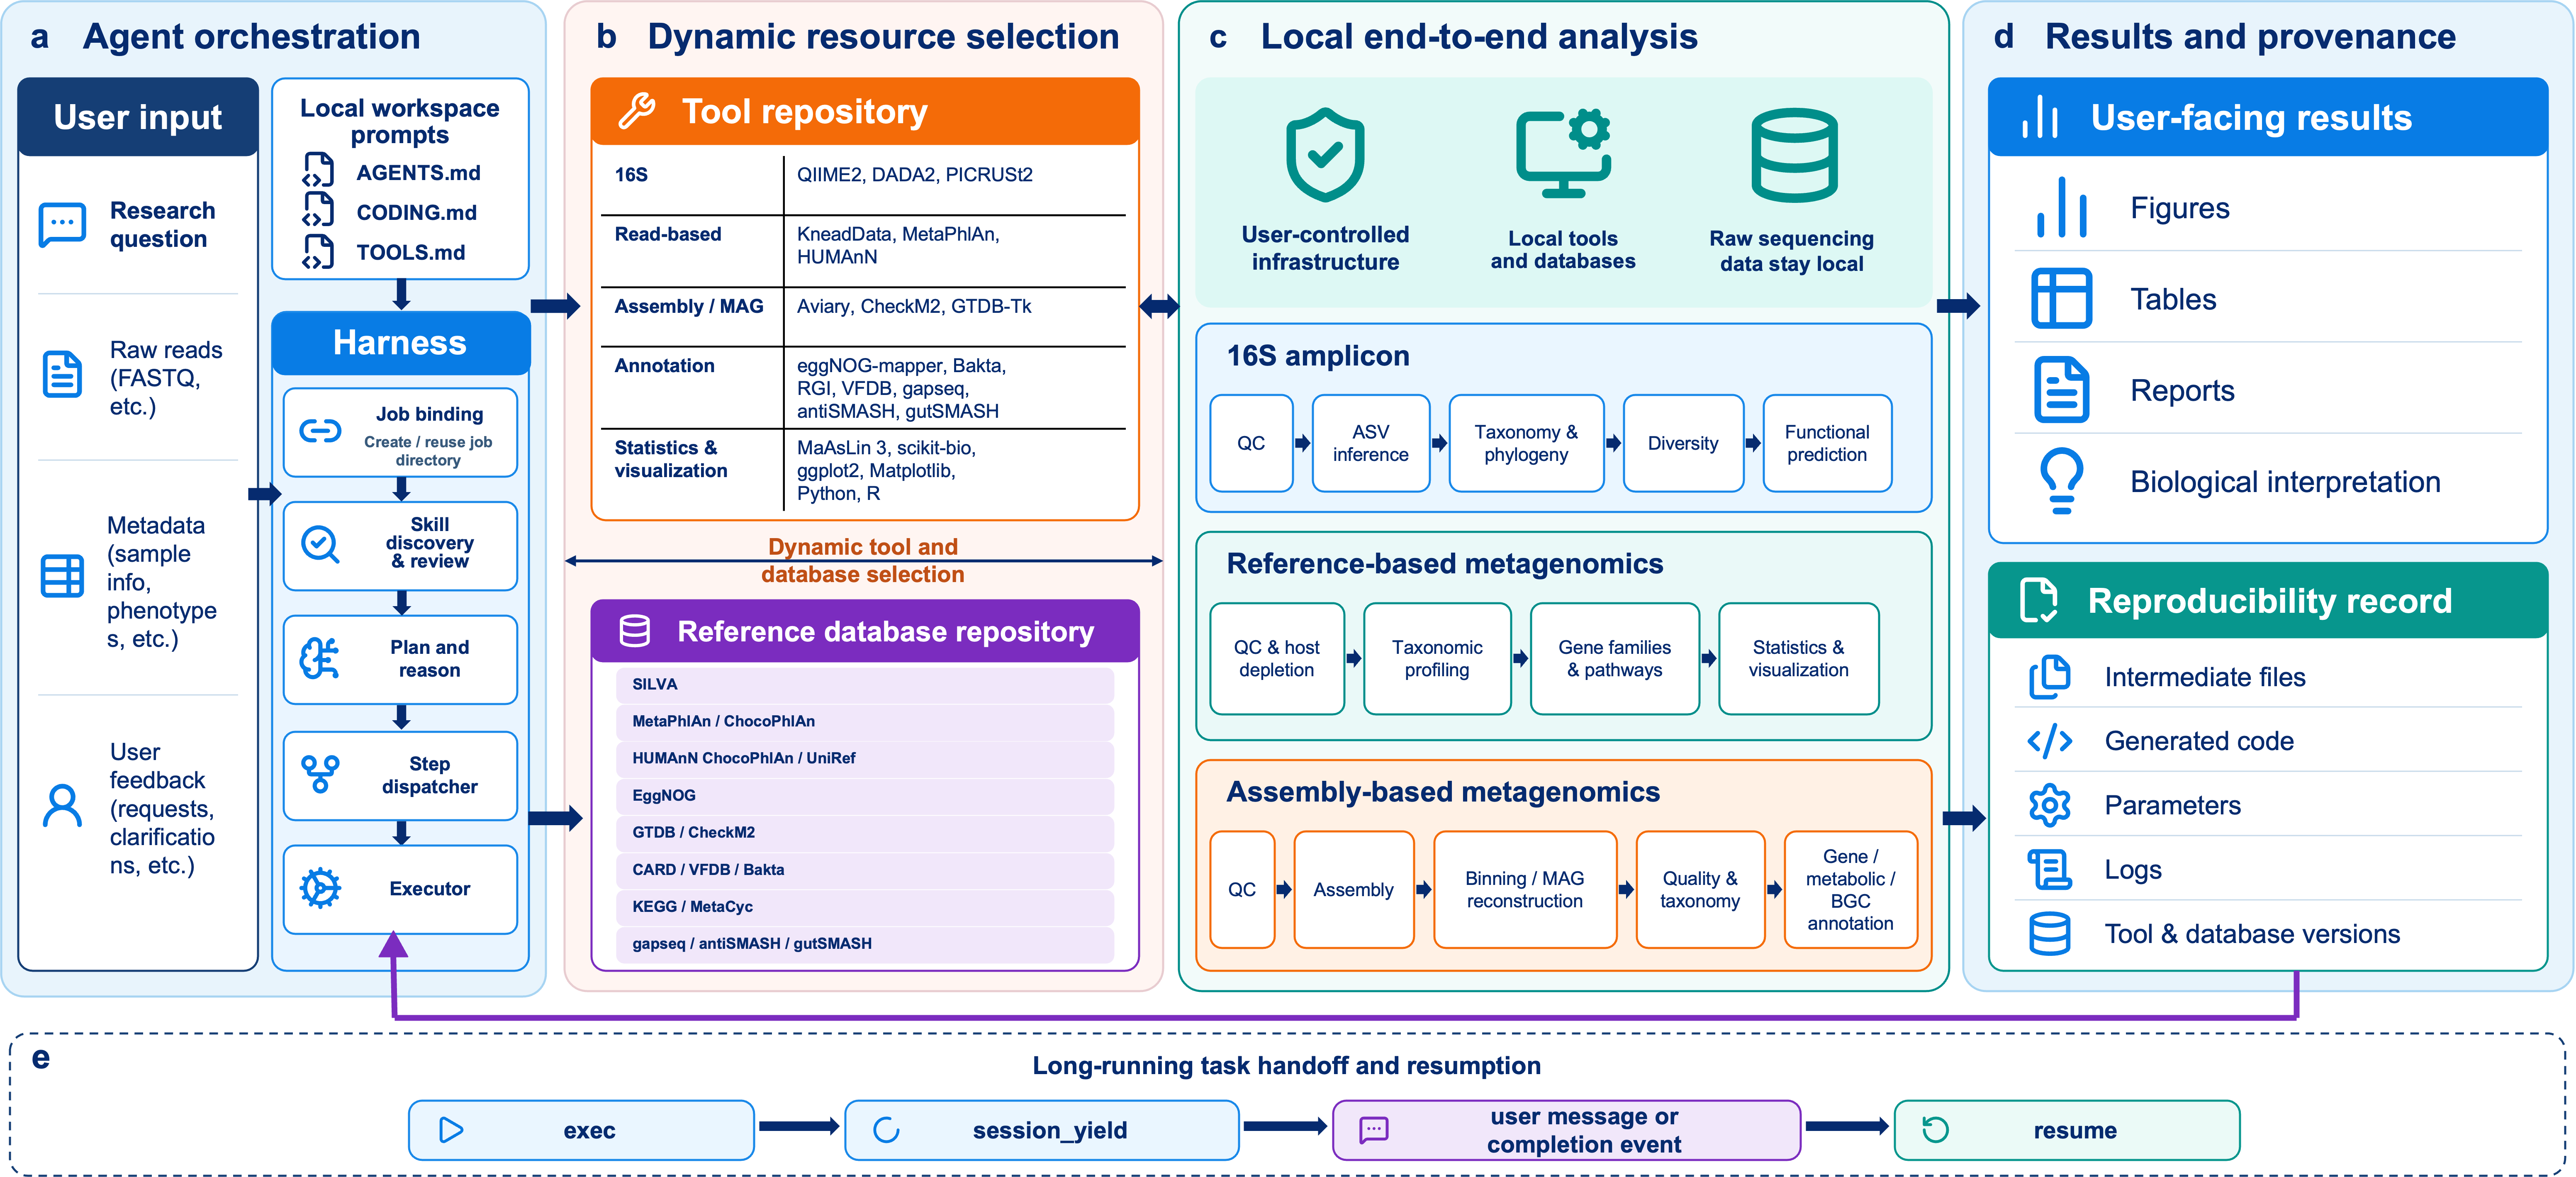
\includegraphics[width=\linewidth]{microbioagent-architecture-image2-v7.png}
\caption{MicroBioAgent architecture and workflow execution. A natural-language
research request initiates an analysis workspace, where the agent formulates an
analytical plan, selects domain-specific skills, and links local software
environments and reference databases across 16S amplicon, reference-based
shotgun, and assembly-based metagenomic workflows. Analysis commands,
parameters, intermediate tables, and logs are organized within the session
directory. During background computation, users can revise pending tasks
without interrupting active processes, and task completion triggers output
verification and continuation within the same session.}
\label{fig:architecture}
\end{figure}

Analytical domain knowledge is modularized into discrete skills, each defined
by a structured \texttt{SKILL.md} document specifying its biological objective,
required inputs, tool dependencies, reference resources, analytical procedures,
and expected deliverables. MicroBioAgent encompasses skills for 16S amplicon
processing (QIIME~2, DADA2), shotgun taxonomic profiling (MetaPhlAn), functional
quantification (HUMAnN), de novo metagenomic assembly and binning (Aviary,
CheckM2), taxonomic placement (GTDB-Tk), coverage calculation (CoverM),
functional annotation (eggNOG-mapper), and downstream statistical analysis
(MaAsLin~3, DESeq2)~\cite{bolyen2019qiime2,callahan2016dada2,%
beghini2021biobakery,newell2026aviary,chklovski2023checkm2,%
chaumeil2022gtdbtk,aroney2025coverm,cantalapiedra2021eggnog,%
huertacepas2019eggnog,nickols2026maaslin3,love2014deseq2}. Software
environments and reference database locations are recorded in two configuration
files. \texttt{runtimes.yaml} identifies the Conda environment containing each
tool or library, whereas \texttt{references.yaml} specifies the locations of
reference databases such as SILVA, ChocoPhlAn, UniRef, and
GTDB~\cite{quast2013silva}.

To execute an investigation, the agent first invokes a dedicated workspace
tool, \texttt{mgx\_create\_job}, which binds the active conversation to an
isolated directory on disk that houses raw inputs, executable scripts,
intermediate tables, and logs throughout the session. Within this workspace,
MicroBioAgent formulates a structured execution plan based on the research
objective, input data, and requested deliverables. The plan defines the
sequence of analytical steps and their completion criteria, maintained directly
within the conversational context. Guided by workspace instructions
(\texttt{AGENTS.md}, \texttt{TOOLS.md}, \texttt{CODING.md}), the agent consults
relevant domain skills to author execution scripts and invoke command-line
utilities via the \texttt{exec} tool. Execution guidelines standardize script 
authoring to balance compute resources across parallel tasks, ensure comprehensive 
logging, and verify that commands execute successfully and produce the expected 
output files. If an execution step fails or expected outputs are missing, the
agent inspects the corresponding logs to diagnose the failure and selectively
rerun the affected analyses.

To accommodate computationally intensive tasks, MicroBioAgent supports
asynchronous background execution with continuous human-in-the-loop
interaction. Analytical commands are launched via \texttt{exec} with an initial
30-second wait period and no overall execution time limit. Commands that finish
within this threshold return their results synchronously. Commands exceeding 30
seconds transition to background processes, prompting the agent to invoke
\texttt{sessions\_yield} to yield its conversational turn. By decoupling
long-running computation from active dialogue, the conversational interface
remains responsive, allowing users to inspect intermediate progress, query the
agent, or adjust pending analysis plans without interrupting active
computations.

To enable automated task resumption after background execution, we implemented
a version-pinned runtime extension for OpenClaw (v2026.7.2) that enhances event
handling and conversation activation. Each background process is tagged with
its originating conversation identifier. When a background task terminates, an
event listener captures the exit status, extracts final log records, and routes
a structured completion notification to the parent session. If the conversation
is idle, the extension immediately initiates a new agent turn without requiring
polling or manual user prompts. If an event arrives during an active
conversational turn, it is placed in a session-specific queue and delivered
once the current turn settles. This design ensures that task results are
reliably processed and analysis continues seamlessly upon process completion.

\section{Experimental design}

\subsection{Study-specific analytical capability}

Three published datasets comprising 230 sequencing libraries assess paired
amplicon and shotgun analysis, colorectal cancer (CRC) functional
classification, and long-read genome-resolved metagenomics
(Table~\ref{tab:cases}). The tomato rhizosphere dataset (PRJNA777724) evaluates
paired amplicon and shotgun profiling across 60 16S (V3--V4) libraries and 36
matched shotgun libraries, spanning four tomato cultivars (two resistant, two
susceptible) across baseline and post-inoculation conditions ($n = 3$
biological replicates per group)~\cite{yin2022tomato}. The CRC dataset
(PRJEB10878) assesses taxonomic and functional profiling across 128 human
faecal shotgun metagenomes from 74 CRC patients and 54
controls~\cite{yu2017crc}. The environmental plastic-degradation dataset
(PRJEB97175) evaluates de novo genome reconstruction using six Oxford Nanopore
long-read metagenomic libraries derived from soil enrichment cultures grown on
low-molecular-weight polyethylene (LMWPE) or alkane
substrates~\cite{sandholm2025polyethylene}. In all three cases, the agent was
powered by \texttt{deepseek-v4-pro} and supplied with raw sequencing reads,
sample metadata, and biological objectives without pre-written execution
scripts. Evaluation examined analytical task completion and the recovery of
primary biological patterns reported in the original studies. Case-study
procedures are detailed in Appendix~\ref{app:case-studies}.

\begin{table}[t]
\centering
\caption{Overview of the three case-study datasets.}
\label{tab:cases}
\normalsize
\setlength{\tabcolsep}{4pt}
\renewcommand{\arraystretch}{1.12}
\begin{tabularx}{\linewidth}{@{}>{\raggedright\arraybackslash}p{0.28\linewidth}l>{\raggedright\arraybackslash}p{0.32\linewidth}>{\raggedright\arraybackslash}X@{}}
\toprule
Case & BioProject & Sequencing libraries & Workflow \\
\midrule
Tomato rhizosphere
  & PRJNA777724
  & 60 16S; 36 matched shotgun
  & 16S and shotgun profiling \\
CRC faecal metagenomes
  & PRJEB10878
  & 128 shotgun
  & Taxonomic and functional profiling \\
Polyethylene enrichment
  & PRJEB97175
  & 6 long-read shotgun
  & Genome-resolved metagenomics \\
\bottomrule
\end{tabularx}
\end{table}

\subsection{Robustness across models and prompts}

To systematically evaluate operational stability while reducing redundant
computational overhead, we evaluated three LLMs (\texttt{deepseek-v4-pro},
\texttt{deepseek-v4-flash}, and \texttt{glm5.3-flash}) crossed with three
prompt complexity levels (Detailed, Medium, Simple), with three independent
sessions per condition ($3 \times 3 \times 3 = 27$ sessions). All runs operated
on shared, preprocessed Case 1 data comprising a 16S ASV table, representative
sequences, a rooted phylogenetic tree, denoising statistics, sample metadata,
and 36 quality-controlled, host-cleared shotgun metagenomic libraries
subsampled to 20\% read depth. The Detailed prompt explicitly prescribed
specific metrics (such as the Shannon index, weighted/unweighted UniFrac,
Bray--Curtis, PERMANOVA, and PERMDISP); the Medium prompt defined analytical
scope but left tool selection to the agent; the Simple prompt stated only the
high-level biological goal~\cite{lozupone2007unifrac,anderson2001permanova}.
Performance was scored across six core tasks: 16S alpha diversity, 16S beta
diversity, 16S genus profiling, 16S
differential abundance, shotgun species profiling, and shotgun differential
abundance. A task was scored as completed when the corresponding quantitative
output was successfully generated. Quantitative consistency was evaluated on
aligned subsets using two-sided Mann--Whitney $U$ tests with Holm correction.
Complete prompts and additional evaluation procedures are provided in
Appendix~\ref{app:evaluation}.

\subsection{Ablation of runtime extension}

Using \texttt{deepseek-v4-pro}, the Detailed Case 1 prompt, and the
preprocessed Case 1 inputs, we conducted three independent replicates under the
full system (\texttt{full}) and three replicates under an ablated configuration
lacking the runtime extension (\texttt{no-patch}). 
In the \texttt{no-patch} configuration, the system lacked automated completion 
notifications, and the agent was not guided to release the conversation 
via \texttt{sessions\_yield}. All other
components---including skills, software environments, and reference
databases---were identical. Sessions ran with no user messages following
initial plan confirmation. Task completion was scored across nine requested
outputs (alpha diversity, beta diversity, 16S genus table, 16S differential
abundance, shotgun species table, shotgun differential abundance, figures,
execution scripts, and an analytical report), and method adherence was
evaluated against the eight diversity and statistical requirements named in the
detailed prompt (sequencing-depth normalization, Shannon diversity, weighted
UniFrac, unweighted UniFrac, Bray--Curtis dissimilarity, weighted-UniFrac PCoA,
PERMANOVA, and PERMDISP). Model calls, tool invocations (\texttt{exec},
\texttt{process}, \texttt{sessions\_yield}), and total token consumption
(input, output, and reasoning tokens) were recorded from full session
transcripts.

\subsection{Interactive guidance during background execution}

To evaluate human-in-the-loop steering, we tested mid-run plan revision while
the Case~1 QIIME~2 taxonomic classification step was running in the background.
Once the classification process was confirmed active, a standardized user
message instructed the agent to keep the running classification command, switch
the subsequent 16S differential-abundance method to DESeq2, and generate a
heatmap of significant genera upon completion, with no further user input
thereafter. Each session was evaluated on two criteria: (1)~whether the agent
processed the instruction and updated the pending analysis plan while the
background process remained active; and (2)~whether the session automatically
resumed upon process completion to inspect outputs and execute the revised plan
without manual user prompting. Three independent sessions were evaluated under
both the \texttt{full} and \texttt{no-patch} configurations.

\section{Results}

\subsection{Study-specific analytical capability}

We first evaluated MicroBioAgent on paired 16S amplicon and shotgun metagenomic
datasets from a tomato rhizosphere bacterial-wilt resistance
study~\cite{yin2022tomato}. Starting from raw reads, the agent executed quality
filtering, DADA2 denoising, taxonomic classification against SILVA 138.2, and
diversity analyses. Consistent with the original study, pathogen inoculation
caused a marked decline in Shannon diversity among susceptible cultivars (A57
and HG70), whereas resistant cultivars (HG64 and HF12) maintained significantly
higher diversity post-inoculation at both day~5 ($P = 0.002$) and day~10
($P = 0.004$; Figure~\ref{fig:tomato}). Weighted-UniFrac PCoA separated samples
primarily by inoculation status along PCoA~1 (56.3\% explained variance),
driven by an expansion of pathogenic \textit{Ralstonia} that dominated
susceptible plants. Differential-abundance analysis using MaAsLin~3 further
identified 6 to 15 genera consistently enriched in resistant cultivars across
sampling conditions (Figure~\ref{fig:tomato-enrichment}). In the matched shotgun metagenomes, profiling with
MetaPhlAn3 identified enrichment of the \textit{Pseudomonas putida} group in
resistant cultivars at baseline (HG64: $P = 0.013$; HF12: $P = 0.009$), but did
not detect the second published marker, \textit{Sphingopyxis unclassified}.
Prompted by this discrepancy, the researcher instructed the agent to re-analyze
the libraries using MetaPhlAn2 (the version used in the original
publication)~\cite{truong2015metaphlan2}. 
This guided reanalysis identified both \textit{P.~putida} ($P < 0.05$) and
\textit{Sphingopyxis unclassified} ($P < 0.1$, matching the source study's
threshold) as enriched in resistant cultivars, recapitulating the
published taxonomic biomarkers.

In the second benchmark, we evaluated MicroBioAgent on a published colorectal
cancer (CRC) cohort comprising 128 human faecal shotgun metagenomes (74 CRC
patients and 54 controls)~\cite{yu2017crc} (Figure~\ref{fig:crc}). Starting from
raw sequencing reads, the agent executed species-level profiling via MetaPhlAn3
and functional quantification of UniRef90 gene families and KEGG Orthology (KO)
groups via HUMAnN3. PCoA of species-level Bray--Curtis dissimilarities showed
no distinct visual separation among controls ($n = 54$), early-stage CRC ($n =
36$), and late-stage CRC ($n = 38$), yet PERMANOVA identified significant
community differences associated with CRC status ($F = 2.32, P = 0.002$) and
disease stage ($F = 1.65, P = 0.009$), whereas clinical covariates (sex, age,
BMI) showed no significant effects. Differential-abundance testing identified
eight CRC-enriched species and two control-enriched species (Benjamini--Hochberg
adjusted $q < 0.05$). Key enriched taxa---\textit{Parvimonas micra},
\textit{Peptostreptococcus stomatis}, \textit{Fusobacterium nucleatum}, and
\textit{Solobacterium moorei}---alongside the control-enriched species
\textit{Eubacterium ventriosum}, exhibited the same direction of association
reported in the original cohort study. A Spearman co-occurrence network
constructed from these ten species revealed 16 positive correlations ($|\rho|
\geq 0.4, q < 0.05$), with \textit{P.~micra} serving as a central hub connected
to six other species, including \textit{F.~nucleatum} ($\rho = 0.49$) and
\textit{S.~moorei} ($\rho = 0.53$). In predictive modeling, the agent
implemented nested fivefold cross-validation with within-fold mRMR feature
selection, training logistic regression classifiers on the top 15
features~\cite{peng2005mrmr}. The gene-family classifier achieved a pooled
out-of-fold AUROC of 0.902 (sensitivity 0.82, specificity 0.89 at Youden's
index), substantially outperforming the KO-based classifier (AUROC 0.632,
sensitivity 0.41, specificity 0.87), confirming that fine-grained gene-family
abundances provided superior diagnostic discrimination.

\begin{figure}[htbp]
\centering
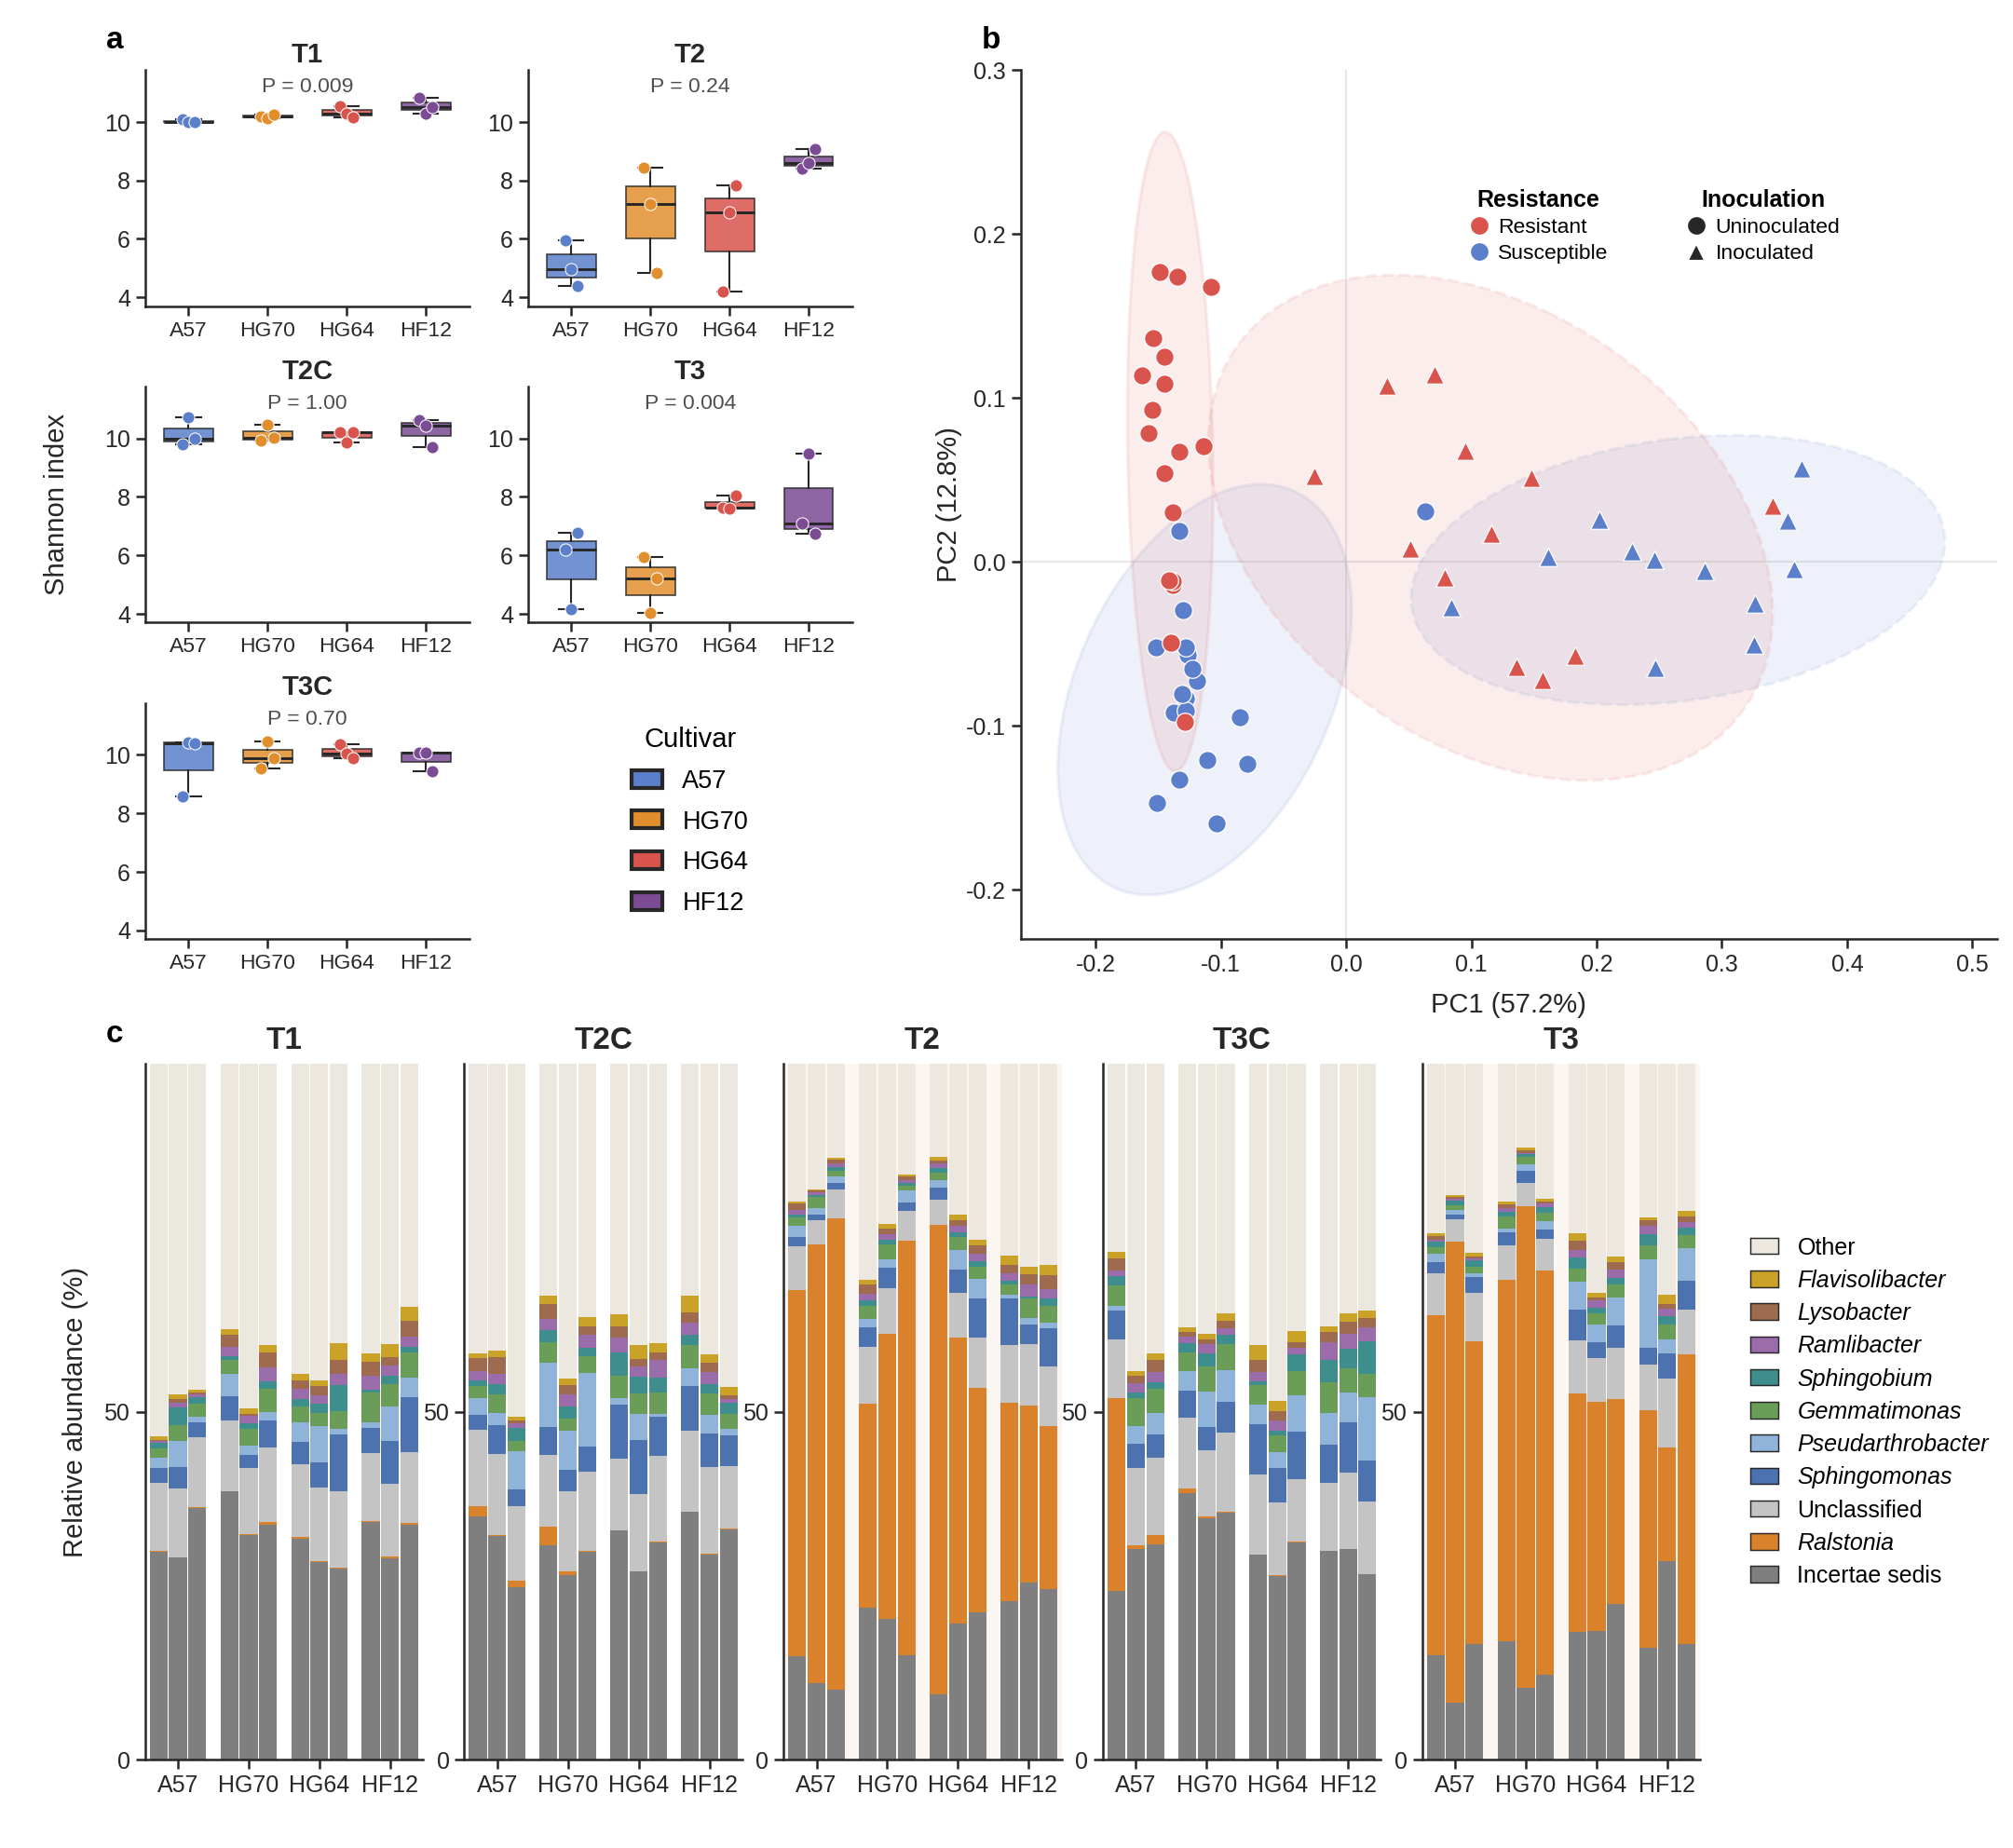
\includegraphics[width=0.60\linewidth]{Case-study-1-Fig1_diversity.png}
\caption{Tomato rhizosphere microbial diversity and community composition.
(a)~Per-sample Shannon diversity across cultivars, sampling timepoints, and
inoculation conditions. (b)~PCoA of weighted UniFrac distances, with samples
colored by resistance phenotype and point shapes indicating inoculation
treatment. (c)~Genus-level relative abundance across individual samples. All
groups contain $n = 3$ biological replicates ($n = 60$ total 16S samples).}
\label{fig:tomato}
\end{figure}

\begin{figure}[htbp]
\centering
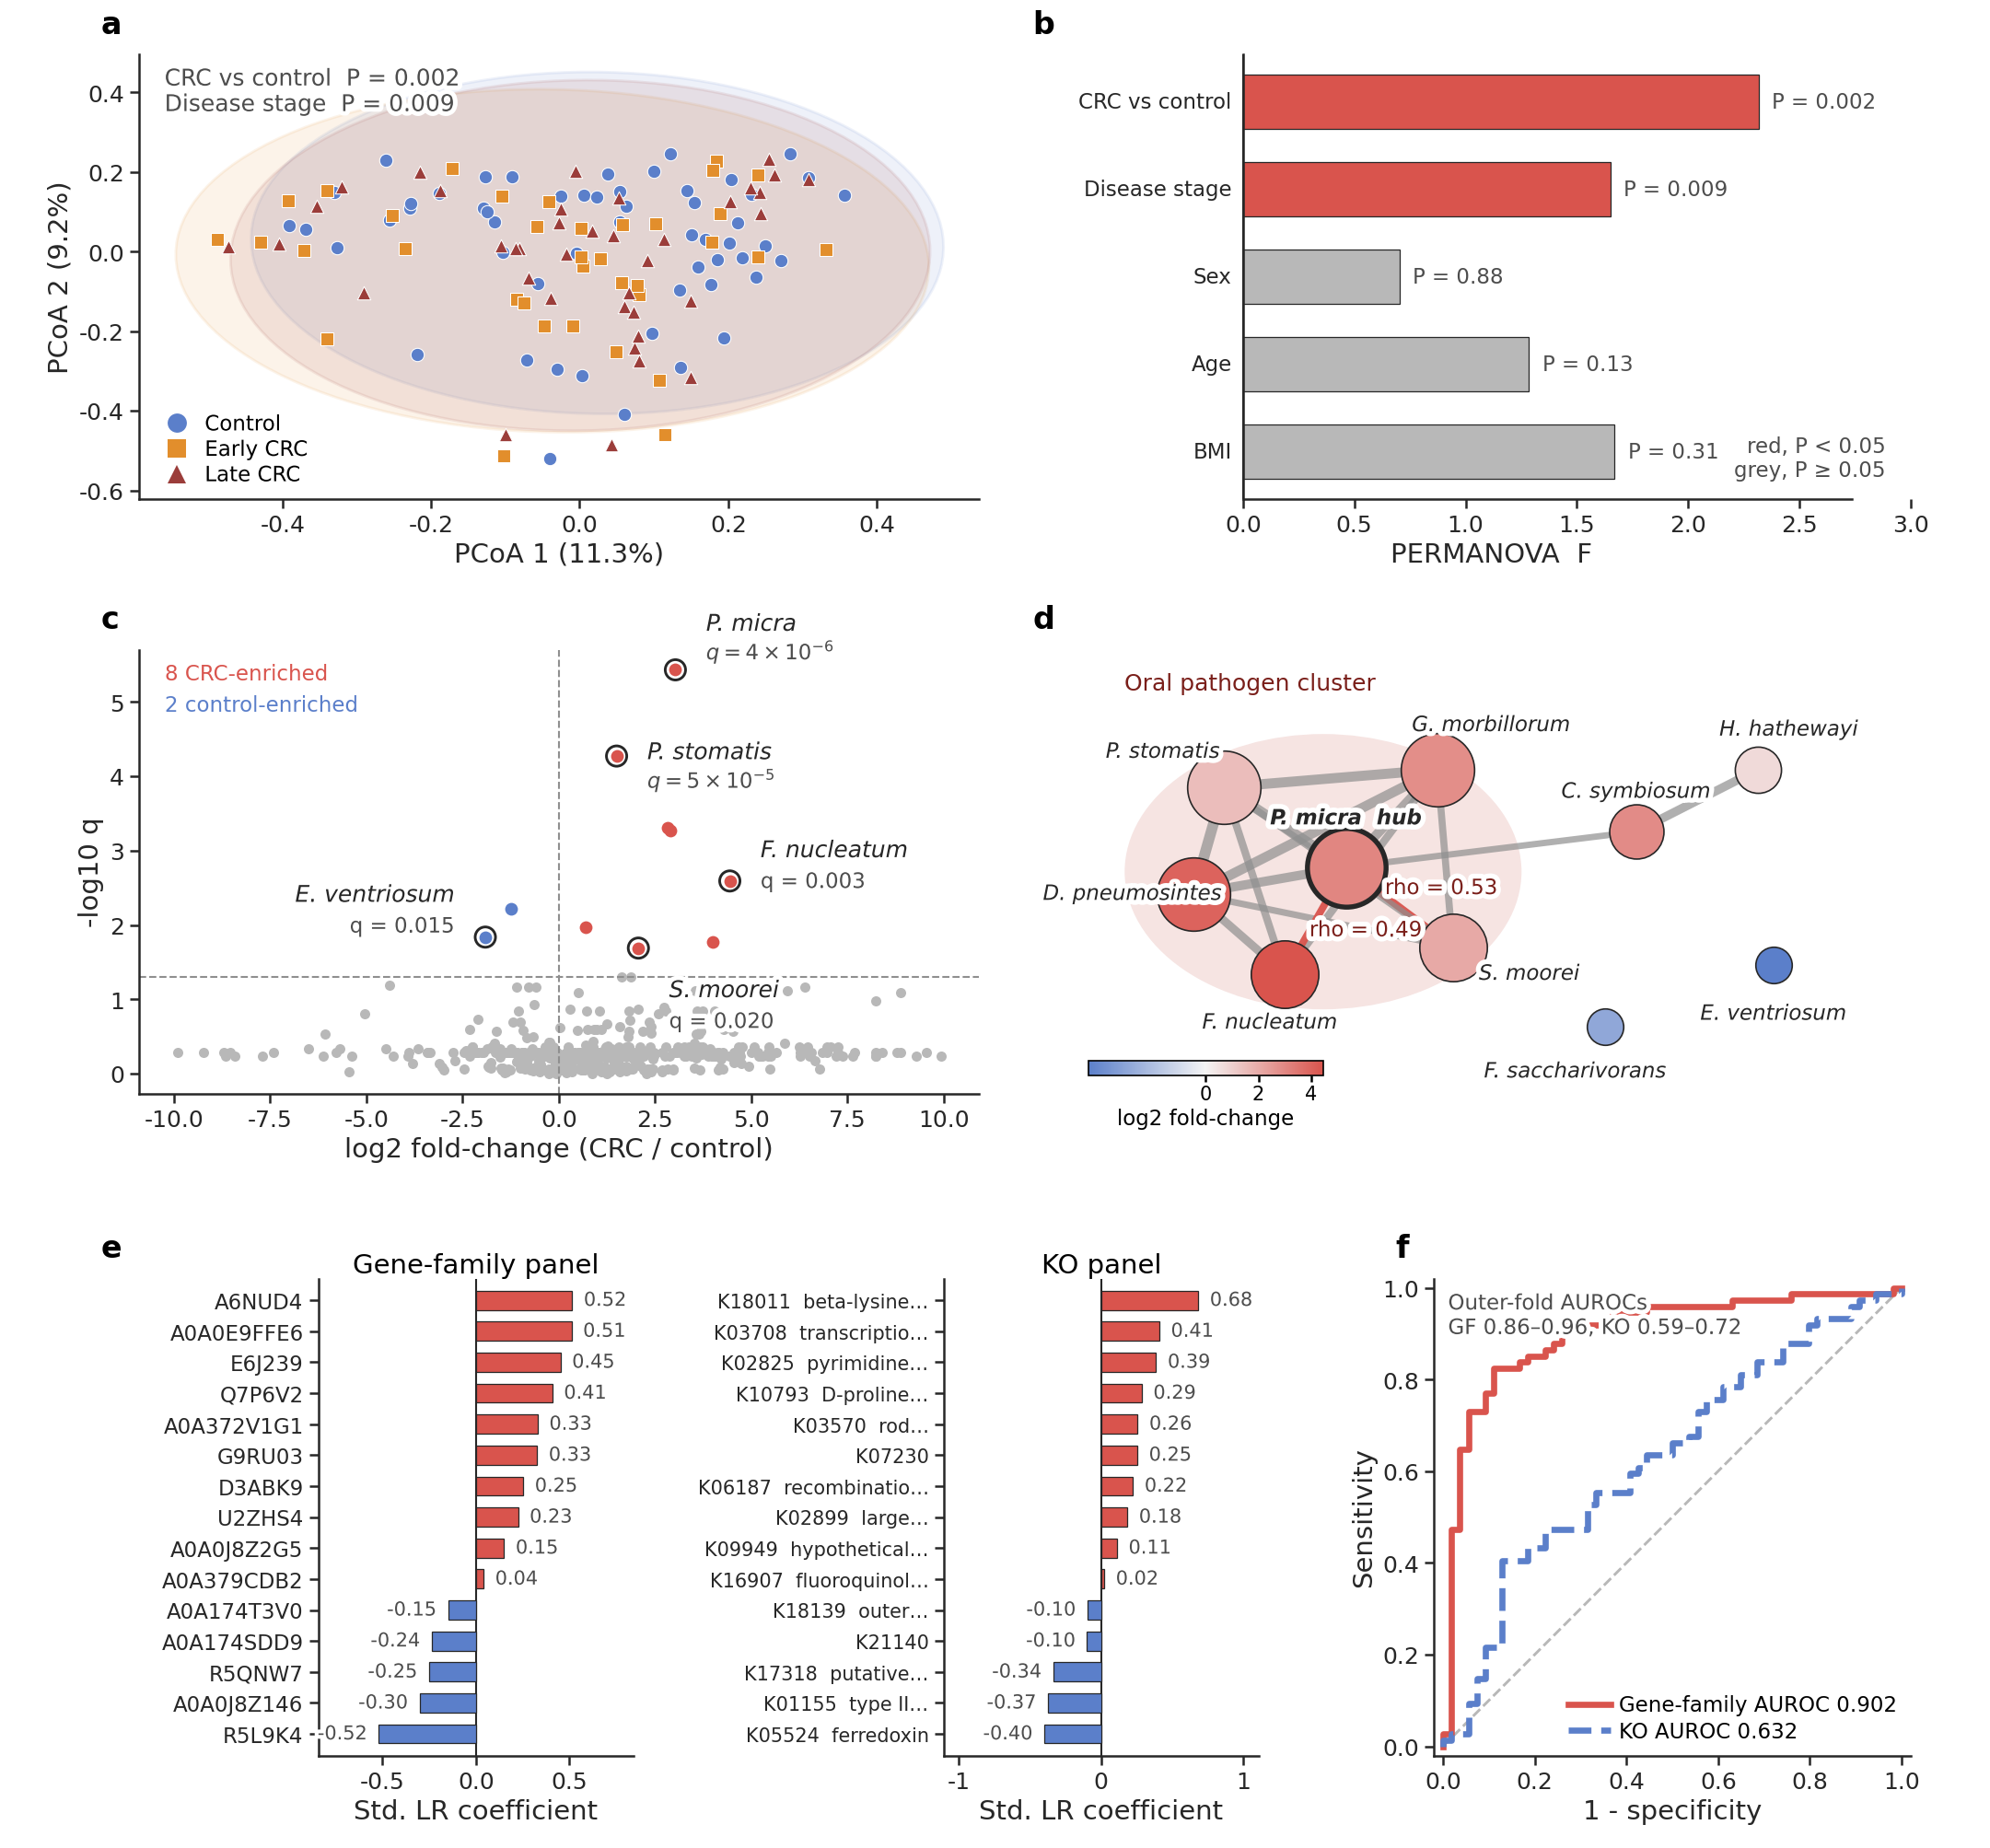
\includegraphics[width=0.60\linewidth]{Case-study-2-Fig_composite.png}
\caption{Metagenomic profiling, biomarker discovery, and predictive modeling in
the CRC cohort. (a)~PCoA of species-level Bray--Curtis dissimilarities across
controls, early-stage CRC, and late-stage CRC cases. (b)~PERMANOVA test
statistics ($F$ values) for disease status, stage, and clinical covariates
(sex, age, and BMI). (c)~Volcano plot of differentially abundant species
between CRC cases and controls (Benjamini--Hochberg adjusted $q < 0.05$).
(d)~Spearman co-occurrence network of the ten differentially abundant species
($|\rho| \geq 0.4$, $q < 0.05$), highlighting the \textit{P.~micra} hub.
(e)~Standardized logistic regression coefficients for the top 15 gene-family
and top 15 KO features selected by mRMR within training folds. (f)~ROC curves
from nested fivefold cross-validation comparing gene-family and KO classifiers.}
\label{fig:crc}
\end{figure}

In the third benchmark, we evaluated MicroBioAgent on de novo genome
reconstruction and metabolic annotation using an environmental
plastic-degradation dataset~\cite{sandholm2025polyethylene}
(Figure~\ref{fig:mag}). The dataset comprised six Oxford Nanopore long-read
metagenomes derived from two soil inocula (S1 and S2) enriched on LMWPE,
triacontane (C30), or tetracontane (C40). Starting from raw long reads, de
novo assembly and binning with Aviary generated 372 initial bins, of which
153 met CheckM2 quality standards (100 high-quality and 53
medium-quality MAGs under MIMAG criteria)%
~\cite{newell2026aviary,chklovski2023checkm2,bowers2017mimag}.
Subsequent dereplication at 95\% average nucleotide identity (ANI) yielded 75
non-redundant representative MAGs (50 high-quality and 25 medium-quality).
Taxonomic assignment via GTDB-Tk (release R232) and relative abundance
estimation via CoverM mapped community structures across carbon sources. In
inoculum S1, \textit{Acinetobacter guillouiae} predominated in LMWPE (64\%)
and C30 (67\%) enrichments, whereas \textit{Aquipseudomonas} dominated C40
(66\% genus-level abundance). In inoculum S2, \textit{Aquipseudomonas}
sp003050835 was most abundant in LMWPE (42\%), \textit{Mesorhizobium\_M}
sp900116595 and \textit{Aquipseudomonas moorei} in C30 (16\% each), and
\textit{Mesorhizobium\_M} sp900116595 and \textit{Aquipseudomonas
fluorescens\_BJ} in C40 (27\% and 25\%, respectively). MicroBioAgent recovered
all ten focal taxonomic groups reported in the original study (with taxa
designated \textit{Pseudomonas} in the original study classified here as
\textit{Aquipseudomonas}, consistent with updated GTDB taxonomic boundaries).
Functional annotation using eggNOG-mapper across 11 representative MAGs of
these focal taxa identified alkane terminal oxidation genes in nine MAGs,
while genes for 2-ketone/oxidized-derivative metabolism and the
$\beta$-oxidation module were detected in all 11 genomes. 

\begin{figure}[htbp]
\centering
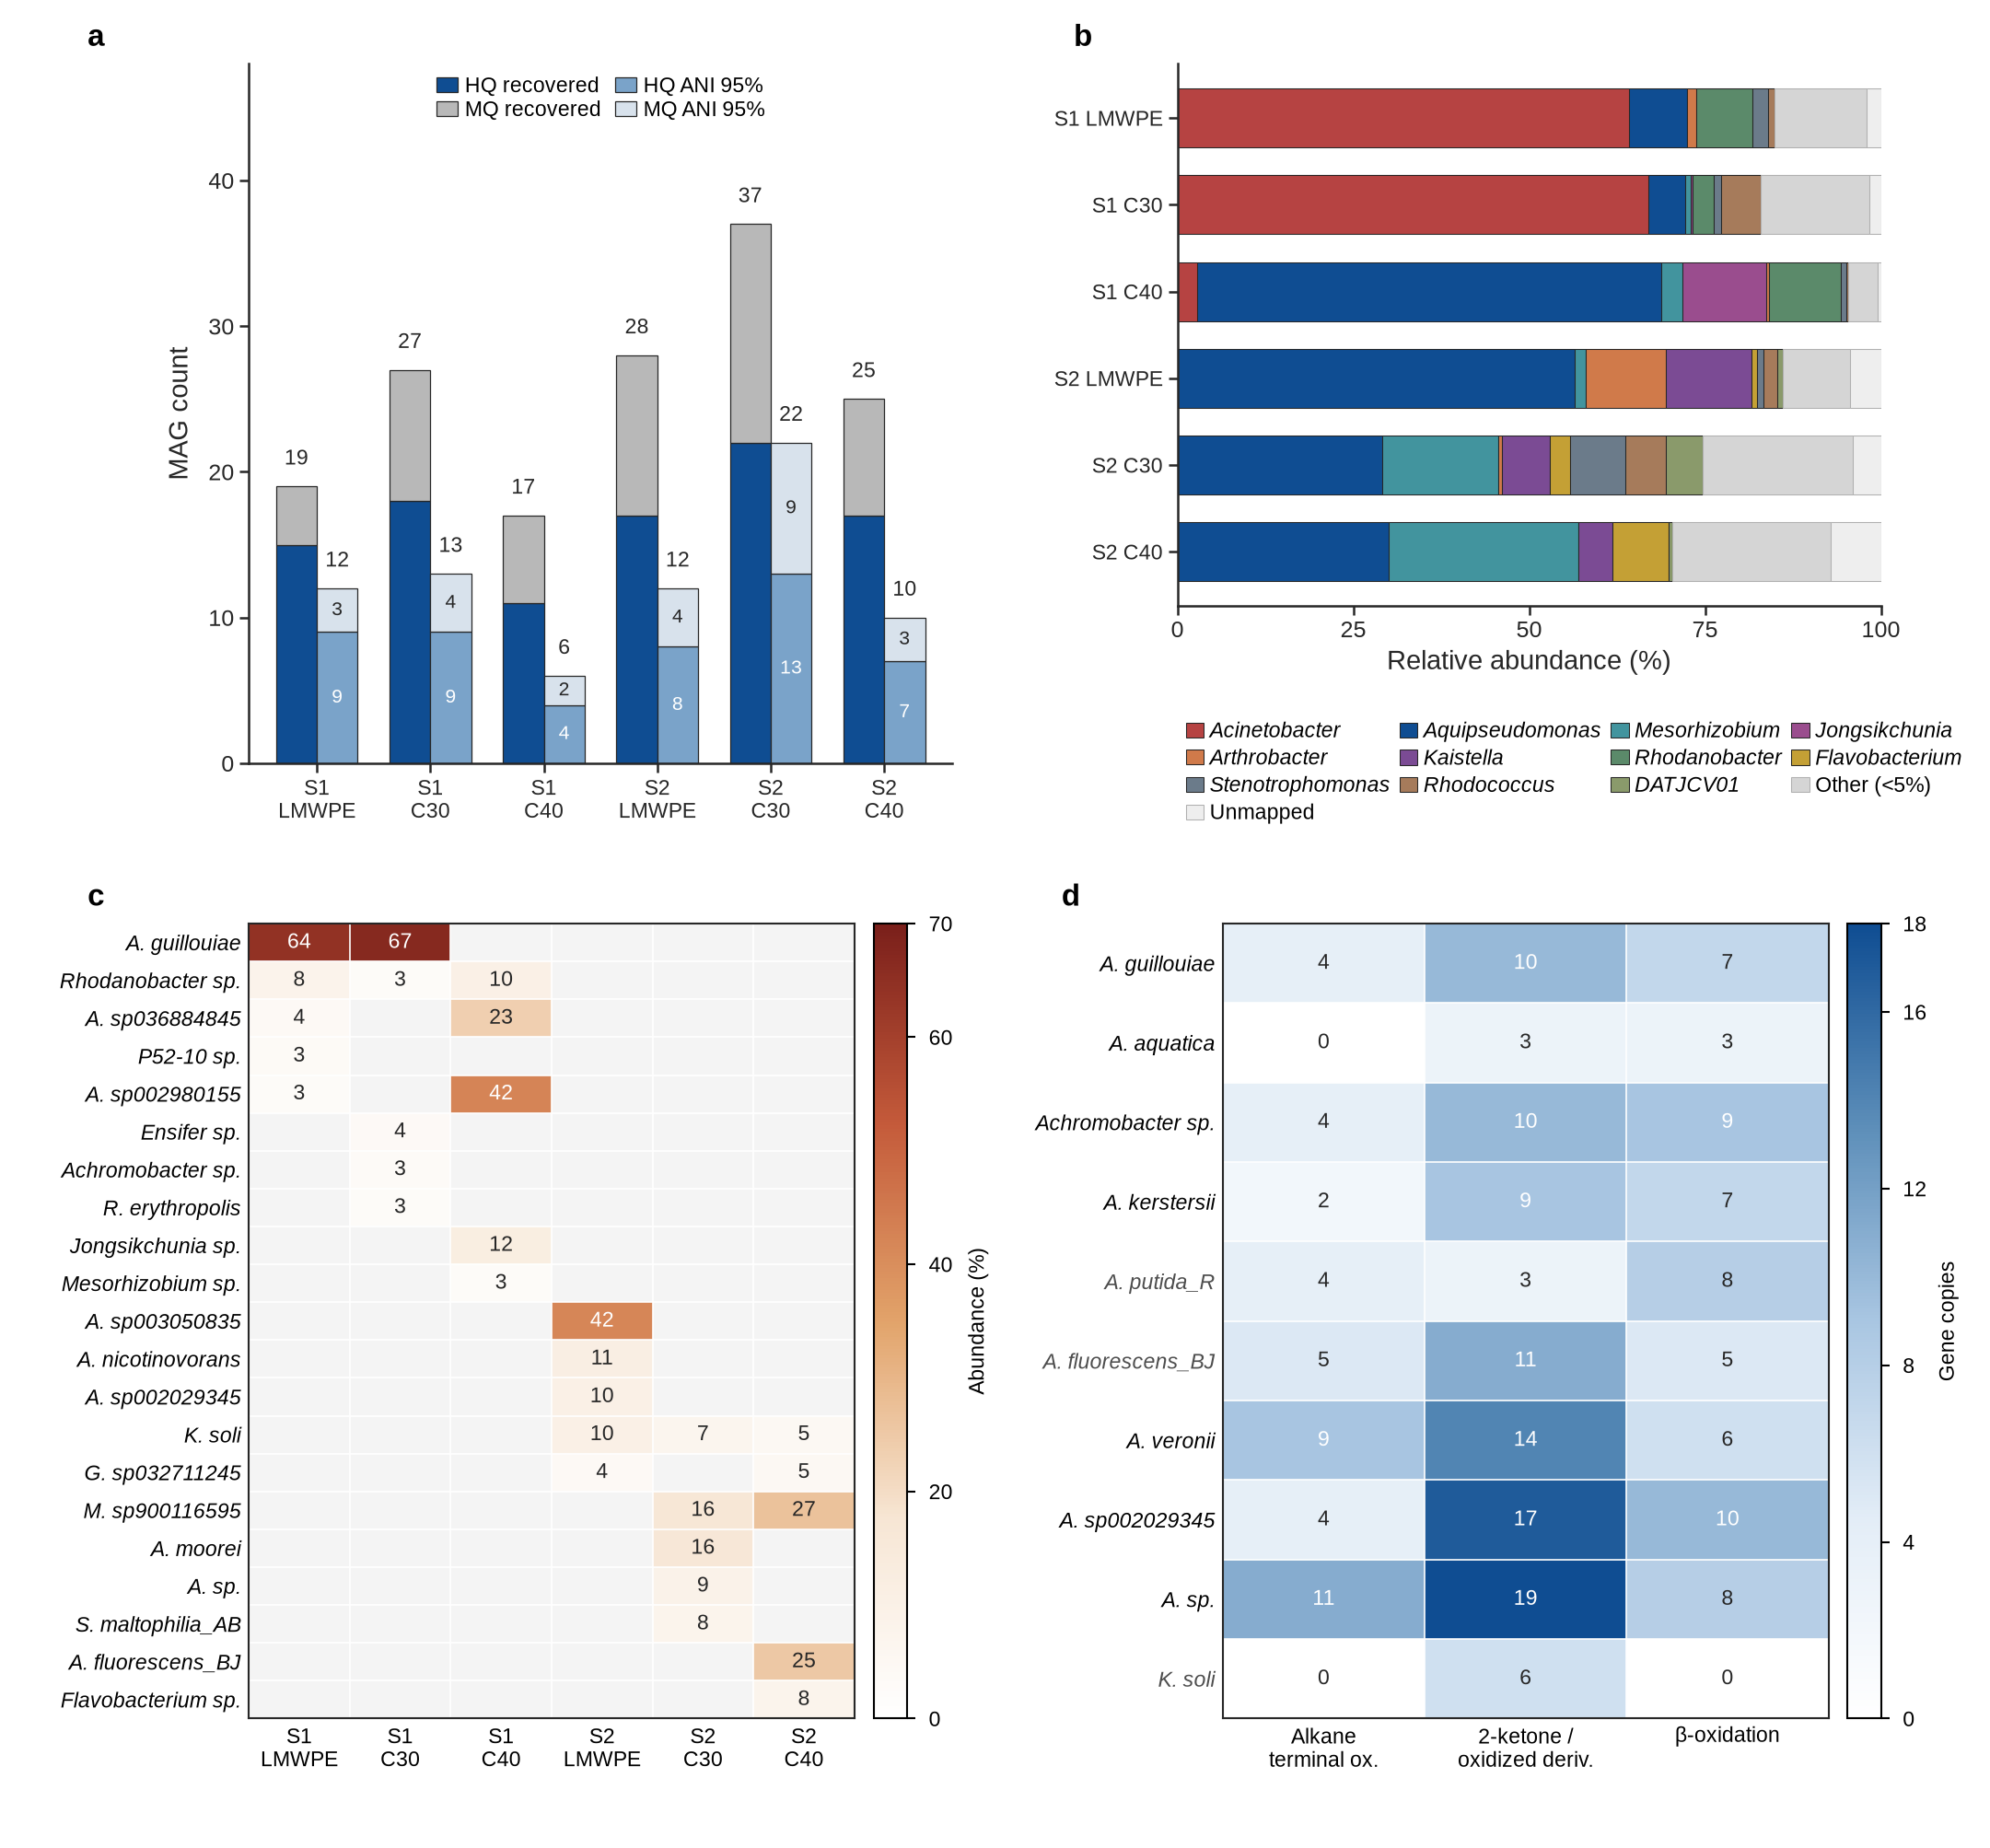
\includegraphics[width=0.78\linewidth]{Case-study-3-Fig_composite.png}
\caption{Genome-resolved metagenomic analysis of polyethylene-enrichment
cultures. (a)~Counts of high-quality (HQ) and medium-quality (MQ) MAGs before
and after 95\% ANI dereplication. (b)~Genus-level relative abundance of MAGs across the
six enrichment cultures. (c)~Relative abundances of species ranked in the top
five of any of the six enrichment cultures. (d)~Gene copy numbers annotated by
eggNOG-mapper in 95\% ANI representative MAGs of focal taxa for alkane terminal
oxidation, 2-ketone or oxidized-derivative metabolism, and $\beta$-oxidation;
taxa in gray font denote medium-quality MAGs.}
\label{fig:mag}
\end{figure}

\subsection{Robustness across models and prompt granularity}

To evaluate whether MicroBioAgent maintains reliable execution and consistent
analytical outputs across LLMs and prompt granularities, we crossed three LLM
backbones (\texttt{deepseek-v4-pro}, \texttt{deepseek-v4-flash}, and
\texttt{glm5.3-flash}) with three prompt levels (Detailed, Medium, and
Simple) on preprocessed Case~1 inputs ($3 \times 3 \times 3 = 27$ independent
sessions) (Figure~\ref{fig:robustness-models}). Across six core analytical
tasks, MicroBioAgent achieved an overall task completion rate of 98.8\% (160
of 162 evaluations). Both \texttt{deepseek-v4-pro} and
\texttt{deepseek-v4-flash} completed all six analyses in three of three
sessions under every prompt level. \texttt{glm5.3-flash} completed all 16S
analyses (9/9 sessions) and 8 of 9 shotgun sessions, omitting the shotgun
workflow in one session under the Detailed prompt. These results demonstrate
that the framework's domain skills and runtime registries provide stable
operational guidance across diverse reasoning backbones and varying degrees
of prompt specification.

Quantitative outputs for community diversity and differential abundance exhibited
broadly concordant distributions across experimental conditions
(Figures~\ref{fig:robustness-models}b and~\ref{fig:robustness-prompts}). Per-sample 16S Shannon diversity
indices (median $9.59\text{--}9.83$) and pairwise weighted UniFrac distances
(median $0.301\text{--}0.303$) showed no statistically significant
differences between any pair of models under any prompt level, or across
prompt levels within any model (all Holm-adjusted $P = 1.0$, two-sided
Mann--Whitney $U$ test). In differential-abundance analyses, individual
sessions autonomously chose among DESeq2, MaAsLin~3, Wilcoxon rank-sum,
Mann--Whitney $U$, or LEfSe~\cite{segata2011lefse}. Restricting cross-model
comparisons to sessions utilizing DESeq2 (Table~\ref{tab:da-model-methods})
revealed no significant
distributional differences in estimated $\log_2$ fold changes across models
(all Holm-adjusted $P \geq 0.059$). Similarly, within-model comparisons
between Detailed and Medium prompts using matched statistical tests
(Table~\ref{tab:da-prompt-methods}) yielded consistent effect-size distributions
(all Holm-adjusted $P \geq 0.064$).

\begin{figure}[htbp]
\centering
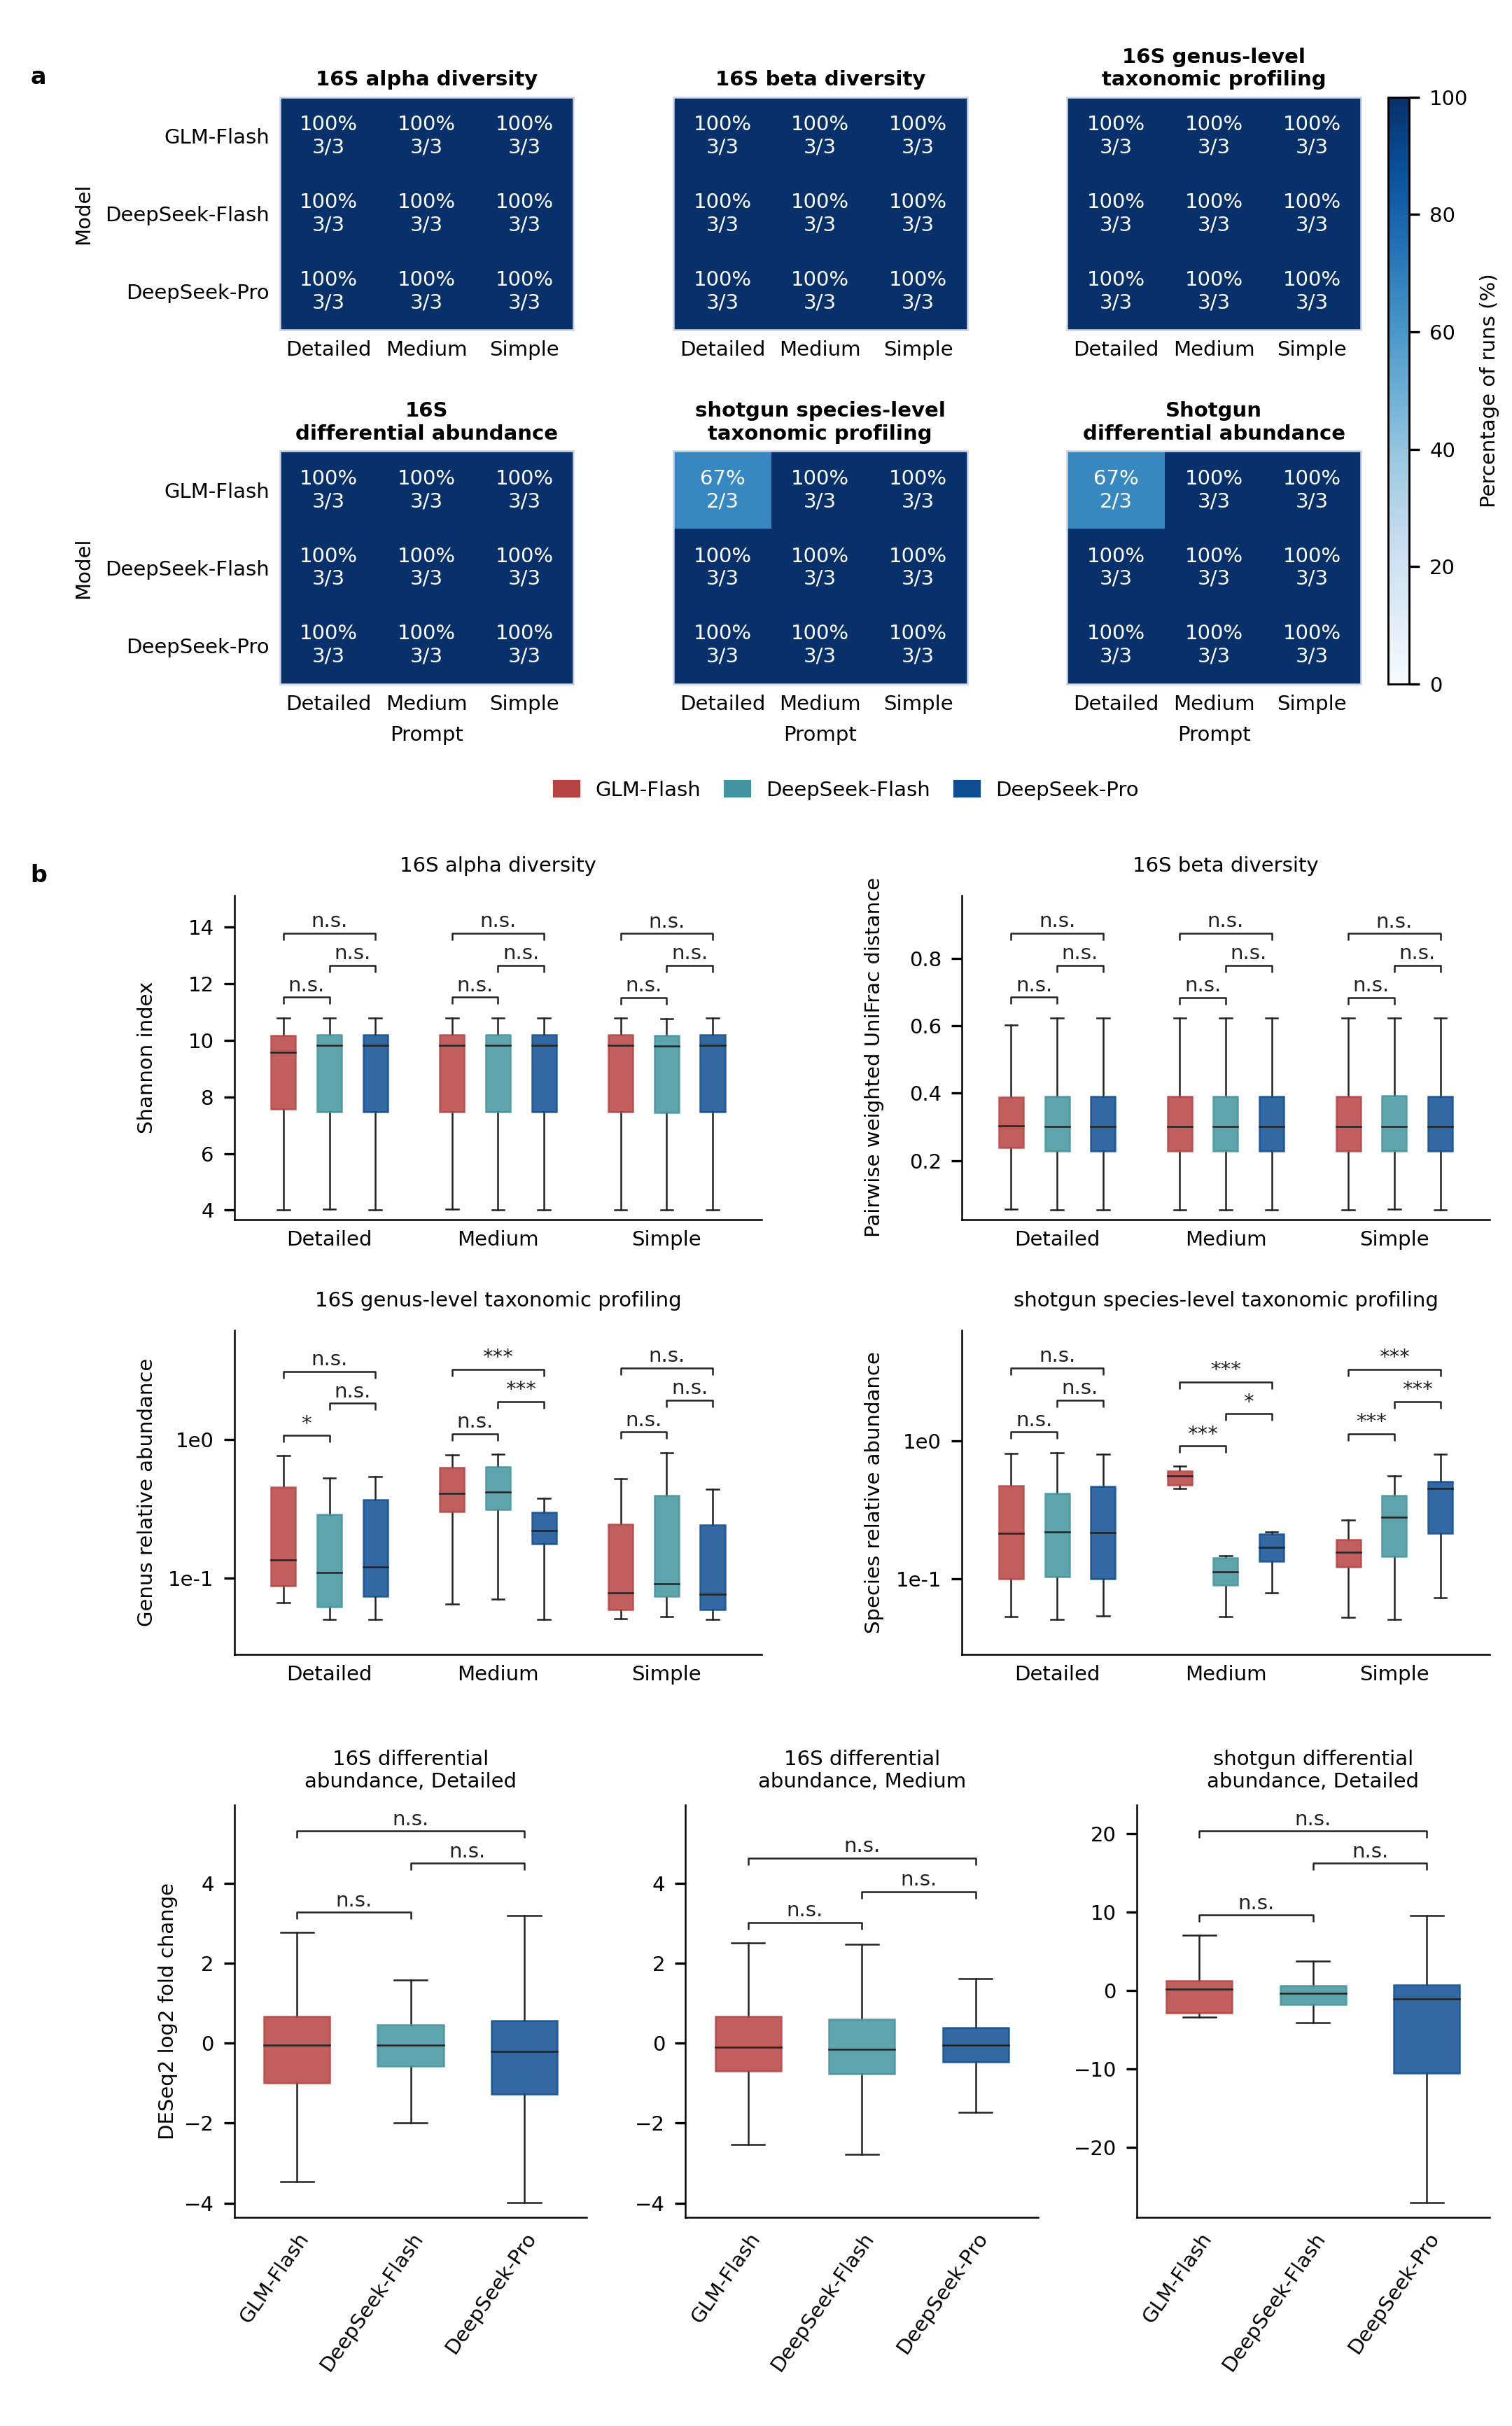
\includegraphics[width=0.62\linewidth]{case1_completion_models.png}
\caption{Overall task completion and differences in analytical outputs across
models within each prompt level. (a)~Completion of six analyses by model and
prompt level; values represent completed sessions out of three. (b)~Comparison
of 16S Shannon diversity indices, pairwise weighted UniFrac distances, and
relative abundances (16S genus level and shotgun species level) among models
under each prompt level, along with DESeq2 $\log_2$ fold changes in taxon
abundance for 16S analyses (detailed and medium prompts) and shotgun analyses
(detailed prompt). Brackets indicate two-sided Mann--Whitney $U$ tests with
Holm correction across the three model pairs in each plot. n.s., adjusted $P
\geq 0.05$; *$P < 0.05$; **$P < 0.01$; ***$P < 0.001$. Values are derived from
repeated analyses of the same Case~1 dataset and do not represent independent
biological replicates.}
\label{fig:robustness-models}
\end{figure}

In contrast, taxonomic relative abundances were more sensitive to model and
prompt specifications. Across models, relative-abundance distributions did
not differ in 16S analyses under the Simple prompt or in shotgun analyses
under the Detailed prompt (all Holm-adjusted $P = 1.0$), but differed in the
remaining settings (Holm-adjusted $P \le 0.05$). Detailed inspection of
session transcripts and generated data matrices revealed three recurring
procedural causes for these differences: (1)~in several 16S amplicon
sessions, the agent selected a V4 rather than a V3--V4 classifier during
taxonomic assignment; (2)~an occasional post-processing script merged sample
abundance tables by row position rather than matching feature identifiers;
and (3)~absent explicit prompt constraints, MetaPhlAn executions differed in
whether the \texttt{--unknown\_estimation} flag was enabled, altering whether
species relative abundances were normalized to total reads or classified
reads. Overall, MicroBioAgent maintained high task completion and consistent
diversity and differential-abundance outputs across models and prompt levels,
with remaining differences largely reflecting choices of analytical tools and
software parameters.

\subsection{Execution efficiency and token consumption}

To evaluate how background task coordination affects execution efficiency and
resource consumption, we compared the full system (\texttt{full}) against the
ablated configuration lacking the runtime extension
(\texttt{no-patch}) across three independent sessions
(Table~\ref{tab:ablation-summary}). Across all replicates, \texttt{full}
produced all 27 requested outputs (9 of 9 per session) and satisfied all 24
prespecified methodological requirements (8 of 8 per session). The
\texttt{no-patch} configuration fulfilled all 24 method requirements
and produced 26 of 27 outputs, omitting only the archived analysis scripts in
a single session. Overall, omitting the runtime extension did
not prevent the agent from completing the requested analyses, but it
fundamentally altered how long-running computations were handled.

In \texttt{full}, whenever a long-running computational command exceeded the
initial 30-second threshold, the agent released conversational control via
\texttt{sessions\_yield} (mean $11.7$ calls per session, range $5\text{--}17$)
to await automated completion notifications, rarely polling process status via
\texttt{process} (mean $7.3$ calls, range $0\text{--}21$, with two sessions
making at most one call). In contrast, the ablated \texttt{no-patch}
configuration never yielded conversational control ($0$ \texttt{sessions\_yield}
calls) and instead repeatedly polled running tasks, issuing an average of
$155.0$ \texttt{process} queries per session (range $102\text{--}227$). Because
each polling round triggered an active model invocation that reprocessed the
expanding conversation transcript, total model calls more than doubled in
\texttt{no-patch} (mean $286.3$, range $211\text{--}403$) compared to
\texttt{full} (mean $133.3$, range $124\text{--}150$). Consequently, mean total
token consumption rose by 141.5\% (a 2.4-fold increase), jumping from
$14.53 \times 10^6$ tokens in \texttt{full} to $35.08 \times 10^6$ tokens in
\texttt{no-patch} (per-session records in Table~\ref{tab:ablation-replicates}).

\begin{table}[t]
\centering
\caption{End-to-end execution ablation and asynchronous steering performance
($n = 3$ independent sessions per condition on preprocessed Case 1).}
\label{tab:ablation-summary}
\normalsize
\setlength{\tabcolsep}{2pt}
\renewcommand{\arraystretch}{1.12}
\begin{tabular*}{\linewidth}{@{\extracolsep{\fill}}lcccccccc@{}}
\toprule
Condition & Outputs & Methods & \shortstack{Model\\calls}
  & \texttt{exec} & \texttt{process} & \texttt{yield}
  & \shortstack{Tokens\\($\times 10^6$)}
  & \shortstack{Steering /\\Resumption} \\
\midrule
\texttt{full} & 27/27 & 24/24 & 133.3 & 82.3 & 7.3 & 11.7 & 14.53 & 3/3 / 3/3 \\
\texttt{no-patch} & 26/27 & 24/24 & 286.3 & 106.0 & 155.0 & 0.0 & 35.08 & 0/3 / 0/3 \\
\bottomrule
\end{tabular*}
\par\vspace{0.4em}
\begin{minipage}{\linewidth}
\normalsize
\textit{Notes:} Conditions include (\texttt{full}) or omit
(\texttt{no-patch}) the runtime patch. All runs used
\texttt{deepseek-v4-pro} with the Detailed prompt. Outputs/methods are pooled
counts; model/tool calls and tokens are per-session means. Total tokens comprise
input and output tokens, including reasoning tokens. The \texttt{yield} column
counts \texttt{sessions\_yield} calls. Steering/resumption give successful
sessions out of three for plan updates while a task runs and automatic
continuation upon completion without further user prompts, respectively.
\end{minipage}
\end{table}

\subsection{Interactive plan revision during background computation}

We next evaluated whether users could interactively revise the pending
analysis plan while a minutes-scale QIIME~2 taxonomic classification command
was running in the background. Once the classification job was confirmed
active, the user sent an instruction to maintain the running process, switch
the subsequent differential-abundance method to DESeq2, and generate a
heatmap of significant genera upon completion.

In \texttt{full}, the agent released conversational control via
\texttt{sessions\_yield} upon starting the task and successfully updated the
pending plan in response to the user's instruction while the classification
job was actively running ($3/3$ sessions; Table~\ref{tab:ablation-summary}).
Once the background process finished, the runtime extension intercepted the
completion event and automatically reactivated the session, allowing the
agent to verify the taxonomic outputs and continue execution under the
revised plan without additional user prompts ($3/3$). In contrast, in the
ablated \texttt{no-patch} configuration, the agent did not release the
dialogue and instead kept the conversation occupied with repeated
\texttt{process} calls. Consequently, neither mid-run plan adjustment nor
automated workflow resumption upon completion was achieved in any of the
replicates ($0/3$).

\section{Discussion}

MicroBioAgent demonstrates that modular domain skills, local software
environments, and event-driven task management can be unified to translate
high-level biological queries into executable microbiome analyses. This
framework is supported by three complementary lines of evidence: (1)~three
diverse case studies establishing flexible end-to-end execution across
amplicon, shotgun metagenomic, and genome-resolved workflows; (2)~systematic
evaluations across 27 independent sessions demonstrating 98.8\% task
completion and reproducible diversity and differential-abundance estimates
across diverse LLMs; and (3)~controlled ablations showing that event-driven
execution reduces token overhead by over 50\% while enabling real-time plan
adjustment. Importantly, MicroBioAgent complements traditional workflow
managers such as Snakemake and Nextflow rather than replacing
them~\cite{koster2012snakemake,ditommaso2017nextflow}. While workflow engines
excel at large-scale, deterministic execution of static pipelines,
MicroBioAgent is tailored for exploratory analyses where analytical plans
must be adaptively formulated, inspected, and refined in response to
intermediate biological findings.

At the same time, our findings highlight that computational execution alone
does not guarantee biological validity. The observed procedural
discrepancies---such as selecting a V4 rather than a V3--V4 classifier,
merging abundance tables by row position rather than matching feature
identifiers, and varying the MetaPhlAn \texttt{--unknown\_estimation}
flag---demonstrate that LLM reasoning remains susceptible to subtle
bioinformatic pitfalls. In the tomato reanalysis, for example, initial
MetaPhlAn3 profiling detected only one of the two reported species markers;
the researcher then specified MetaPhlAn2, the version used in the original
study, which recovered both. This rerun shows that the recovered markers
depended on the software version. Crucially, by preserving executable
commands, parameters, and intermediate tables within an inspectable
workspace, MicroBioAgent makes these analytical decisions transparent,
allowing life scientists to audit each step, diagnose unexpected variations,
and steer downstream analyses accordingly.

Several limitations of the current study warrant further investigation.
First, our robustness and ablation experiments were evaluated on preprocessed
inputs from a single benchmark dataset; future evaluations should examine
operational stability across broader cohort scales and raw sequencing
modalities. Second, while our ablation quantified the operational benefits of
event-driven execution over status polling, the comparison was conducted at
the runtime-extension level; finer-grained component-wise ablations and
direct comparisons against general-purpose coding agents supplied with
identical tools will help isolate the marginal contribution of
domain-specific skills. Nevertheless, MicroBioAgent establishes an
adaptable, auditable paradigm for autonomous computational research, bridging
natural-language biological intent with rigorous, local bioinformatic
execution.

\section{Conclusion}

MicroBioAgent establishes an autonomous, domain-specific framework for
end-to-end computational microbiome research. By integrating modular
analytical skills, local software environments, and reference registries, the
framework translates natural-language biological goals into executable
multi-stage workflows without relying on hardcoded pipeline templates.
Furthermore, its background task management mechanism decouples
long-running bioinformatics computations from conversational dialogue,
reducing token overhead by over 50\% while enabling seamless, interactive
human steering and automated workflow resumption. Across diverse plant,
clinical, and environmental datasets, MicroBioAgent demonstrates high
analytical robustness and biological concordance, providing a scalable,
transparent foundation for autonomous microbiome analysis.

\section*{Code and data availability}

Code, skills, prompts, environment specifications, and the version-pinned
runtime patch are publicly available at \url{https://github.com/Zeming-LI-Andy/openclaw-microbiome}.
Raw sequencing reads are publicly available under BioProject accessions
PRJNA777724 (tomato rhizosphere), PRJEB10878 (CRC cohort), and PRJEB97175
(polyethylene enrichment). The LLMs were accessed through Volcano Engine.

\clearpage
\bibliographystyle{unsrt}
\bibliography{../refs}

\clearpage
\appendix
\renewcommand{\thefigure}{A\arabic{figure}}
\renewcommand{\thetable}{A\arabic{table}}
\setcounter{figure}{0}
\setcounter{table}{0}
\raggedbottom

\section{Supplementary methods and results}
\label{app:supplementary}

\subsection{Implementation and reproducibility}
\label{app:implementation}

Software and database versions used across the case studies are listed in
Table~\ref{tab:software-versions}.

\begin{table}[H]
\centering
\caption{Principal software tools and reference databases used across the three
  case studies.}
\label{tab:software-versions}
\normalsize
\setlength{\tabcolsep}{6pt}
\renewcommand{\arraystretch}{1.12}
\begin{tabularx}{\linewidth}{@{}>{\raggedright\arraybackslash}p{0.36\linewidth}>{\raggedright\arraybackslash}X@{}}
\toprule
Software or reference database & Version or release \\
\midrule
QIIME~2 & 2024.10.1 \\
DADA2 & 1.30.0; QIIME~2 plugin 2024.10.0 \\
SILVA 138.2 & 138.2 \\
KneadData & 0.12.4; \texttt{hg37dec\_v0.1} \\
MetaPhlAn & 3.0.7; \texttt{mpa\_v30\_CHOCOPhlAn\_201901} \\
MetaPhlAn & 2; \texttt{mpa\_v20\_m200} \\
HUMAnN & 3.0.0.alpha.4; ChocoPhlAn \texttt{v296\_201901} \\
MaAsLin3 & 1.2.0 \\
Aviary & 0.13.2; assembler myloasm 0.3.0 \\
CheckM2 & 1.1.0 \\
CoverM & 0.7.0 \\
GTDB-Tk & 2.7.2; database R232 \\
eggNOG-mapper & 2.1.13; eggNOG 5.0.2 \\
\bottomrule
\end{tabularx}
\end{table}

\subsection{Case-study details and extended results}
\label{app:case-studies}

The tomato rhizosphere samples (PRJNA777724~\cite{yin2022tomato}) covered five
sampling conditions. These were baseline (T1), inoculated day~5 (T2),
uninoculated control day~5 (T2C), inoculated day~10 (T3), and uninoculated
control day~10 (T3C). Figure~\ref{fig:tomato-enrichment} provides genus-level
MaAsLin~3 comparisons for the resistant cultivars.

The CRC classifiers used $L_2$-regularized logistic regression, with feature
selection and model fitting confined to each training fold before held-out
evaluation.

% Keep the extended tomato figure with the case-study details.
\begin{figure}[H]
\centering
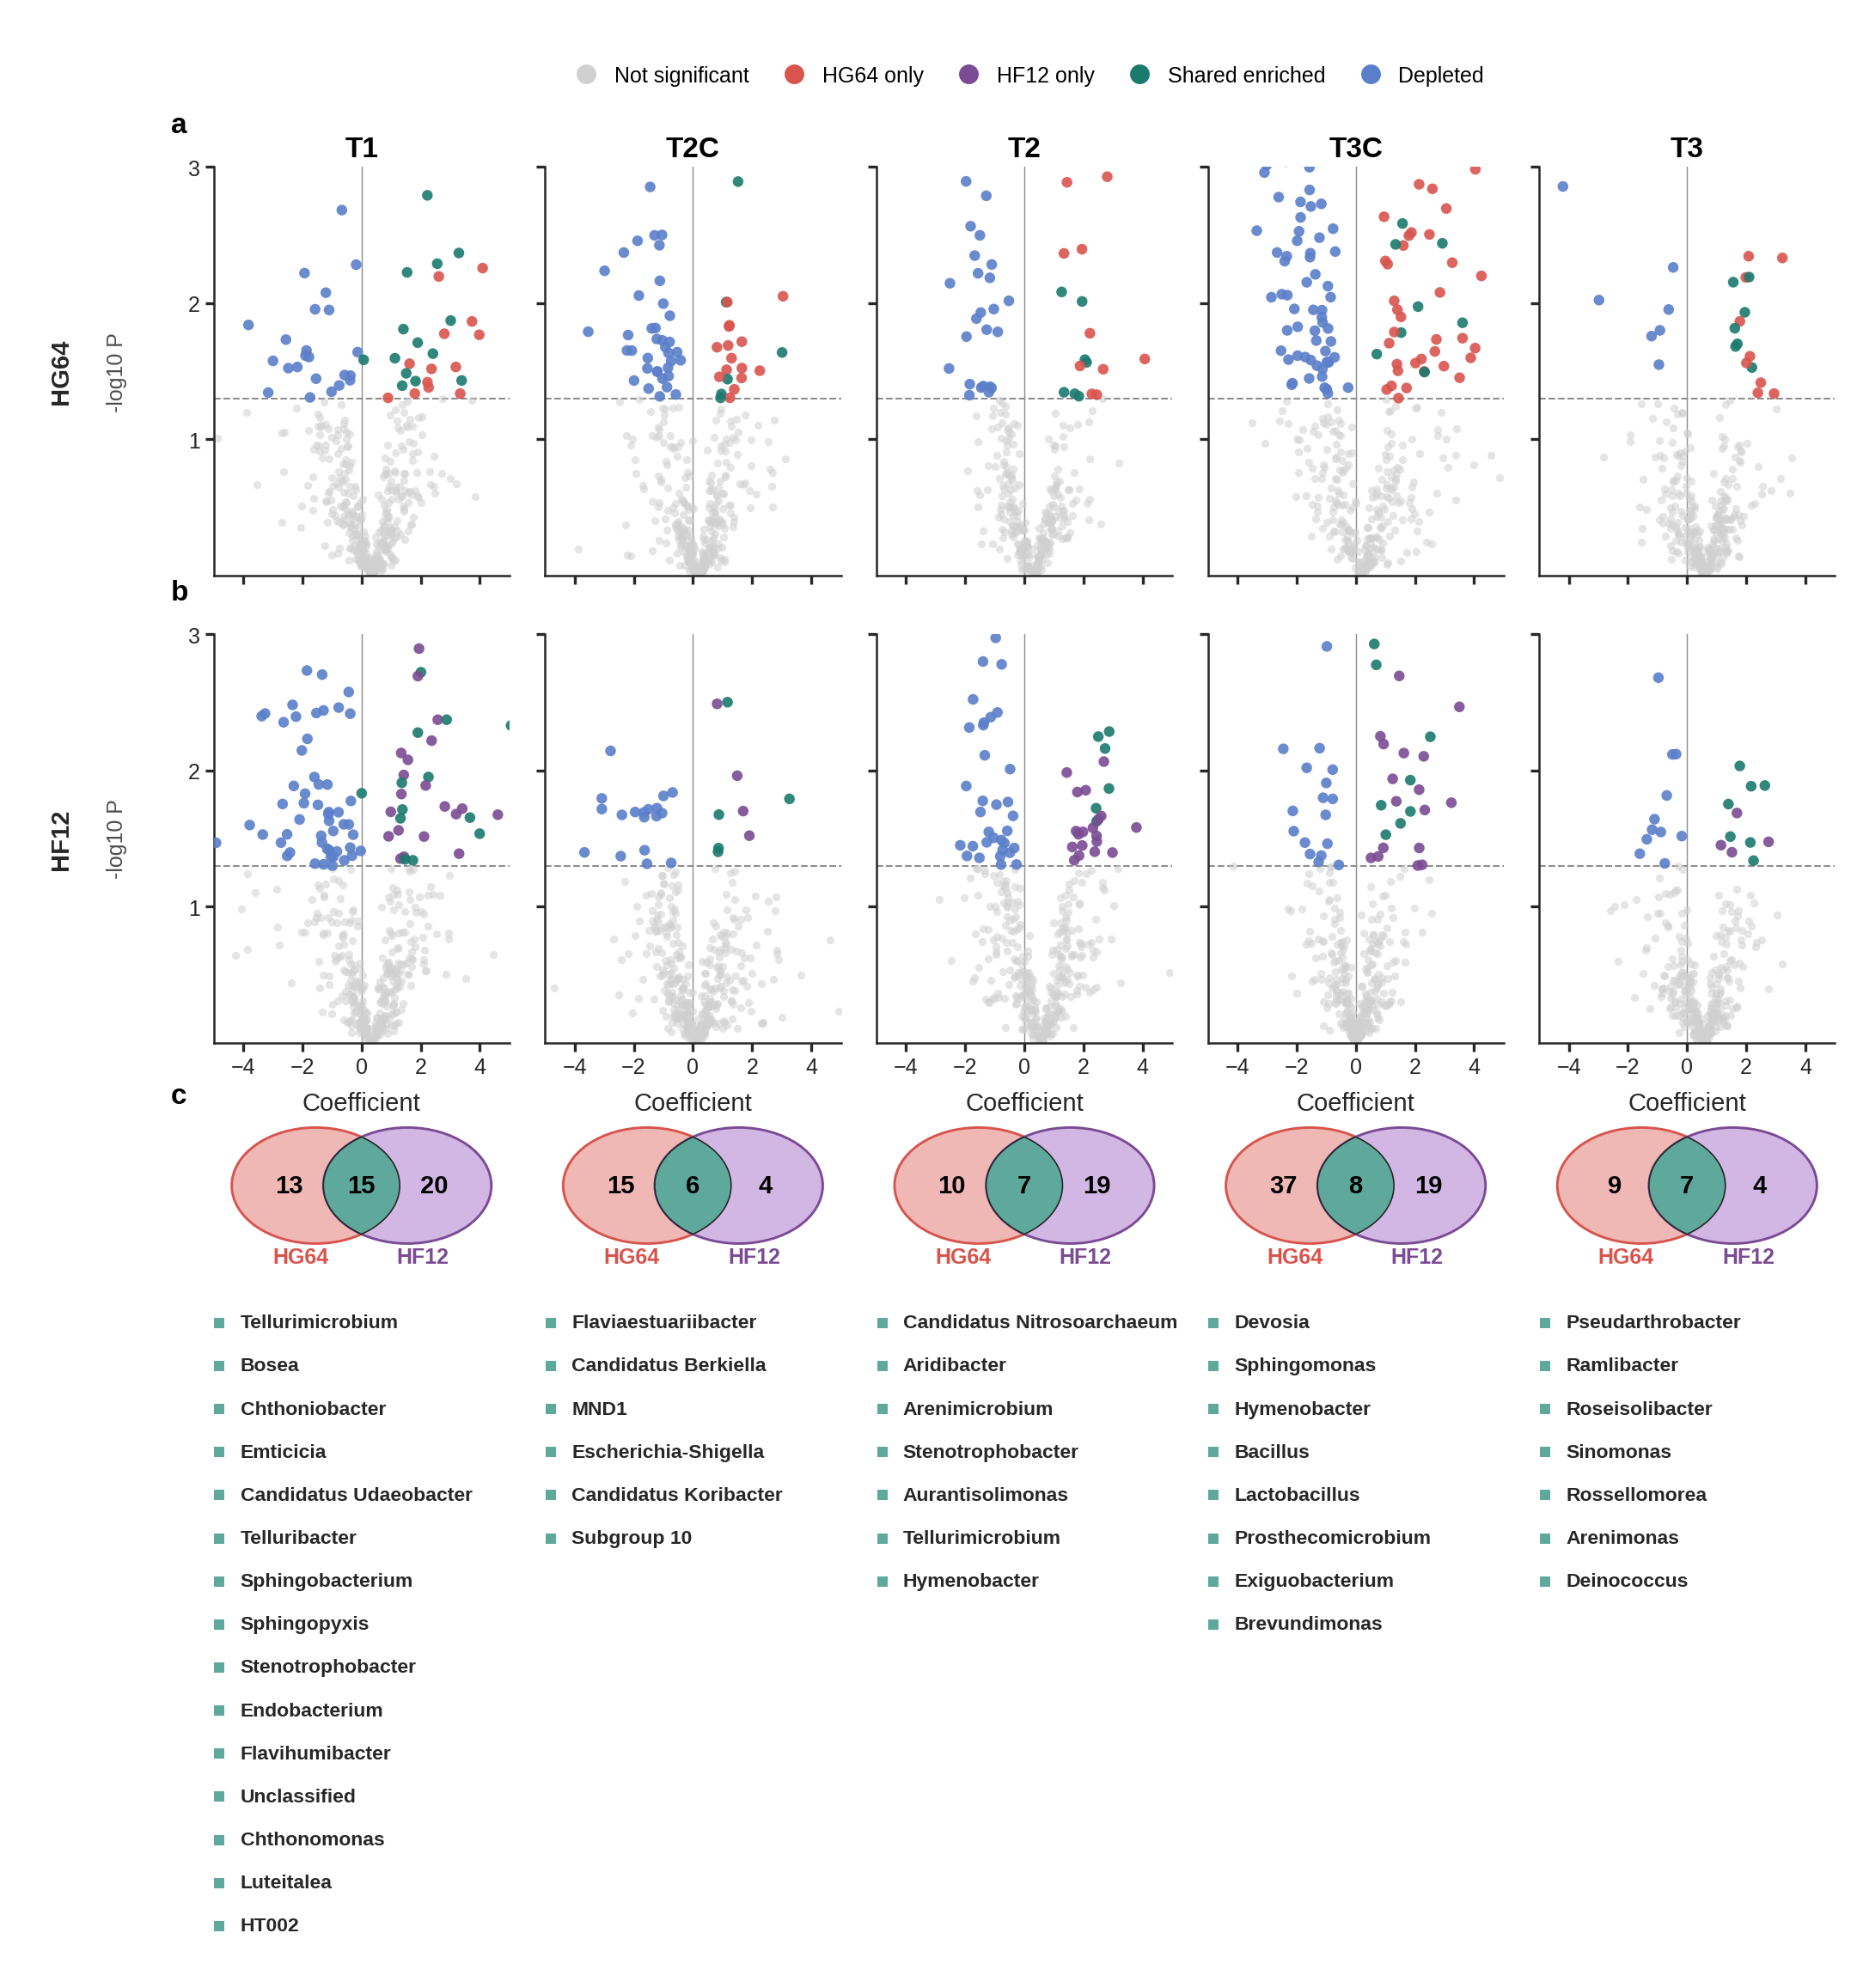
\includegraphics[width=0.94\linewidth]{Case-study-1-Fig2_16s_genus_enrichment.png}
\caption{Genus-level differential abundance in the 16S profiles of the resistant
  tomato parent HG64 and the resistant F1 hybrid HF12. (a,~b)~Volcano plots of
  MaAsLin~3 coefficients for HG64 (a) and HF12 (b) versus the pooled susceptible
  cultivars at each sampling condition. (c)~Overlap of genera with a positive
  coefficient and $P<0.05$ in both resistant cultivars.}
\label{fig:tomato-enrichment}
\end{figure}

\clearpage
\subsection{Additional evaluation details}
\label{app:evaluation}

The full Detailed, Medium, and Simple prompts used in the robustness evaluation
are reproduced below.

% Tighten list spacing without changing the 10 pt text size.
\renewenvironment{promptitems}{%
  \begin{itemize}%
  \setlength{\itemsep}{0pt}%
  \setlength{\parsep}{0pt}%
  \setlength{\topsep}{0.15em}%
  \setlength{\leftmargin}{1.2em}%
}{\end{itemize}}
\tcbset{before upper={\normalsize\setlength{\parskip}{0.15em}},
  title after break={Detailed prompt (continued)}}
\begin{promptbox}{Detailed prompt}
You are provided with rhizosphere shotgun metagenomic data and matched 16S rRNA
gene amplicon data from a tomato bacterial-wilt experiment. Conduct a
comprehensive exploratory and comparative microbiome analysis covering both 16S
rRNA and shotgun metagenomic profiling.
\prompthead{Data Characterization and Quality Control}
\begin{promptitems}
\item Describe all available metadata variables and the hierarchical structure
  of the dataset: cultivar genotype, resistance phenotype, sampling timepoint,
  inoculation treatment, biological replicate.
\item Visualize the experimental design, sequencing depth, and QC retention
  using sample-flow diagrams and distribution plots stratified by cultivar,
  timepoint, and treatment.
\end{promptitems}
\prompthead{16S rRNA Alpha Diversity Analysis}
\begin{promptitems}
\item Calculate Shannon diversity for each sample from the post-QC, non-chimeric
  ASV feature table after sequencing-depth normalization.
\item At each sampling timepoint, compare Shannon diversity among cultivars and
  between resistant and susceptible phenotype groups.
\item Visualize Shannon diversity with box/violin plots by cultivar and
  resistance phenotype, faceted by timepoint and treatment.
\end{promptitems}
\prompthead{16S rRNA Beta Diversity Analysis}
\begin{promptitems}
\item Quantify between-sample dissimilarity from the post-QC ASV feature table
  using \textbf{Weighted UniFrac}, \textbf{Unweighted UniFrac}, and
  \textbf{Bray--Curtis}.
\item Visualize weighted-UniFrac PCoA with samples colored by phenotype and
  shaped or faceted by cultivar, timepoint, and treatment.
\item Use PERMANOVA to assess resistance phenotype, cultivar, inoculation
  treatment, sampling timepoint, and prespecified interaction terms. Assess
  homogeneity of multivariate dispersion with PERMDISP before interpreting
  PERMANOVA.
\end{promptitems}
\prompthead{16S Taxonomic Profiling and Differential Abundance Analysis}
\begin{promptitems}
\item Conduct taxonomic classification and abundance-composition analysis.
\item At each independent sampling timepoint, identify taxa with significantly
  different abundances between each resistant focal cultivar and the susceptible
  control group.
\item Screen and summarize microbial markers significantly enriched in both
  resistant cultivars \textbf{HG64} and \textbf{HF12} at \textbf{T1},
  \textbf{T2C}, and \textbf{T2}. Define these shared taxa as core
  resistance-associated biomarkers.
\item Visualize composition with stacked bar plots and differential taxa with
  volcano plots or heatmaps; summarize shared biomarkers with an UpSet plot.
\end{promptitems}
\tcbbreak
\prompthead{Shotgun Metagenome Taxonomic and Differential Abundance Analysis}
\begin{promptitems}
\item Perform species-level taxonomic annotation and abundance profiling.
\item At each independent sampling timepoint, identify taxa with significantly
  different abundances between each resistant focal cultivar and the susceptible
  control group.
\item Screen and summarize markers significantly enriched in both \textbf{HG64}
  and \textbf{HF12} at \textbf{T1}, \textbf{T2C}, and \textbf{T2} as core
  resistance-associated biomarkers.
\item Visualize species-level composition with stacked bar plots and
  differential species with volcano plots or heatmaps; summarize shared markers
  with an UpSet plot.
\end{promptitems}
\end{promptbox}

\tcbset{title after break={Medium prompt (continued)}}
\begin{promptbox}{Medium prompt}
You are provided with rhizosphere shotgun metagenomic data and matched 16S rRNA
gene amplicon data from a tomato bacterial-wilt experiment. Conduct a
comprehensive exploratory and comparative microbiome analysis covering both 16S
rRNA and shotgun metagenomic profiling.
\prompthead{Data characterization}
\begin{promptitems}
\item Describe the dataset structure and assess quality.
\item Visualize experimental design, sequencing depth, and QC, stratified by
  cultivar, timepoint, and treatment.
\end{promptitems}
\prompthead{16S diversity, taxonomy, and differential abundance}
\begin{promptitems}
\item Compare alpha and beta diversity among cultivars and between resistant and
  susceptible groups, stratified by timepoint.
\item Profile taxonomic composition.
\item At each timepoint, identify taxa that differ between each resistant focal
  cultivar and the susceptible control.
\item Identify markers enriched in both \textbf{HG64} and \textbf{HF12} at
  \textbf{T1}, \textbf{T2C}, and \textbf{T2}.
\end{promptitems}
\prompthead{Shotgun taxonomy and differential abundance}
\begin{promptitems}
\item Profile species-level composition.
\item At each timepoint, identify species that differ between each resistant
  focal cultivar and the susceptible control.
\item Identify markers enriched in both \textbf{HG64} and \textbf{HF12} at
  \textbf{T1}, \textbf{T2C}, and \textbf{T2}.
\end{promptitems}
\end{promptbox}

\tcbset{title after break={Simple prompt (continued)}}
\begin{promptbox}{Simple prompt}
You are provided with rhizosphere shotgun metagenomic data and matched 16S rRNA
gene amplicon data from a tomato bacterial-wilt experiment. Analyze the dataset
and identify microbiome patterns associated with wilt resistance, using both 16S
and shotgun profiles.
\end{promptbox}

% Keep the comparison methods and their two supporting tables together.
\clearpage
Analytical outputs were averaged across completed replicate sessions and aligned
on shared entries before comparison. Diversity comparisons included per-sample
Shannon indices ($n = 60$) and pairwise weighted UniFrac distances ($n =
1{,}770$). Taxonomic abundance comparisons used shared sample--taxon entries
with a session-mean relative abundance of at least 5\% in every compared group.
This filter limited the influence of fluctuations in rare taxa on rank-based
comparisons. Differential-abundance comparisons included all shared taxa without
an abundance threshold and were restricted to sessions using identical
statistical software (Tables~\ref{tab:da-model-methods}
and~\ref{tab:da-prompt-methods}; Figure~\ref{fig:robustness-prompts}).

\begin{table}[H]
\centering
\caption{Replicate sessions and shared entries for cross-model DESeq2
  comparisons.}
\label{tab:da-model-methods}
\normalsize
\setlength{\tabcolsep}{5pt}
\renewcommand{\arraystretch}{1.12}
\begin{tabularx}{\linewidth}{@{}>{\raggedright\arraybackslash}Xlcccc@{}}
\toprule
Dataset & Prompt
  & \shortstack{DeepSeek\\Pro}
  & \shortstack{DeepSeek\\Flash}
  & \shortstack{GLM\\Flash}
  & \shortstack{Shared\\entries} \\
\midrule
16S rRNA gene, genus & Detailed & 1/3 & 2/3 & 3/3 & 1,724 \\
16S rRNA gene, genus & Medium & 1/3 & 2/3 & 1/3 & 2,659 \\
Shotgun metagenome, species & Detailed & 1/3 & 2/3 & 2/3 & 228 \\
\bottomrule
\end{tabularx}
\par\vspace{0.4em}
{\normalsize Values for each model indicate the number of independent replicates
  (out of three) that selected DESeq2. Shared entries are the taxa evaluated
  across all three models. Shotgun results under the medium prompt were not
  compared because no single differential-abundance method was selected by all
  three models.}
\end{table}

\begin{table}[H]
\centering
\caption{Replicate sessions and shared entries for prompt-level
  differential-abundance comparisons.}
\label{tab:da-prompt-methods}
\normalsize
\setlength{\tabcolsep}{6pt}
\renewcommand{\arraystretch}{1.12}
\begin{tabular}{@{}llccc@{}}
\toprule
Model & Method
  & \shortstack{Detailed\\sessions}
  & \shortstack{Medium\\sessions}
  & \shortstack{Shared\\entries} \\
\midrule
\multicolumn{5}{@{}l}{\textit{16S rRNA gene, genus}} \\
\addlinespace
\texttt{deepseek-v4-pro} & DESeq2 & 1/3 & 1/3 & 891 \\
\texttt{deepseek-v4-flash} & DESeq2 & 2/3 & 2/3 & 5,108 \\
\texttt{glm5.3-flash} & DESeq2 & 3/3 & 1/3 & 3,984 \\
\addlinespace
\multicolumn{5}{@{}l}{\textit{Shotgun metagenome, species}} \\
\addlinespace
\texttt{deepseek-v4-pro} & Wilcoxon & 1/3 & 1/3 & 39 \\
\texttt{deepseek-v4-flash} & Mann--Whitney $U$ & 1/3 & 1/3 & 120 \\
\texttt{glm5.3-flash} & DESeq2 & 2/3 & 1/3 & 52 \\
\bottomrule
\end{tabular}
\par\vspace{0.4em}
{\normalsize Session counts indicate the number of independent replicates (out
  of three) that selected the specified statistical method under each prompt
  level. Shared entries are the taxa evaluated across both prompt levels.}
\end{table}

% Keep this comparison figure before the execution-ablation material.
\clearpage
\begin{figure}[H]
\centering
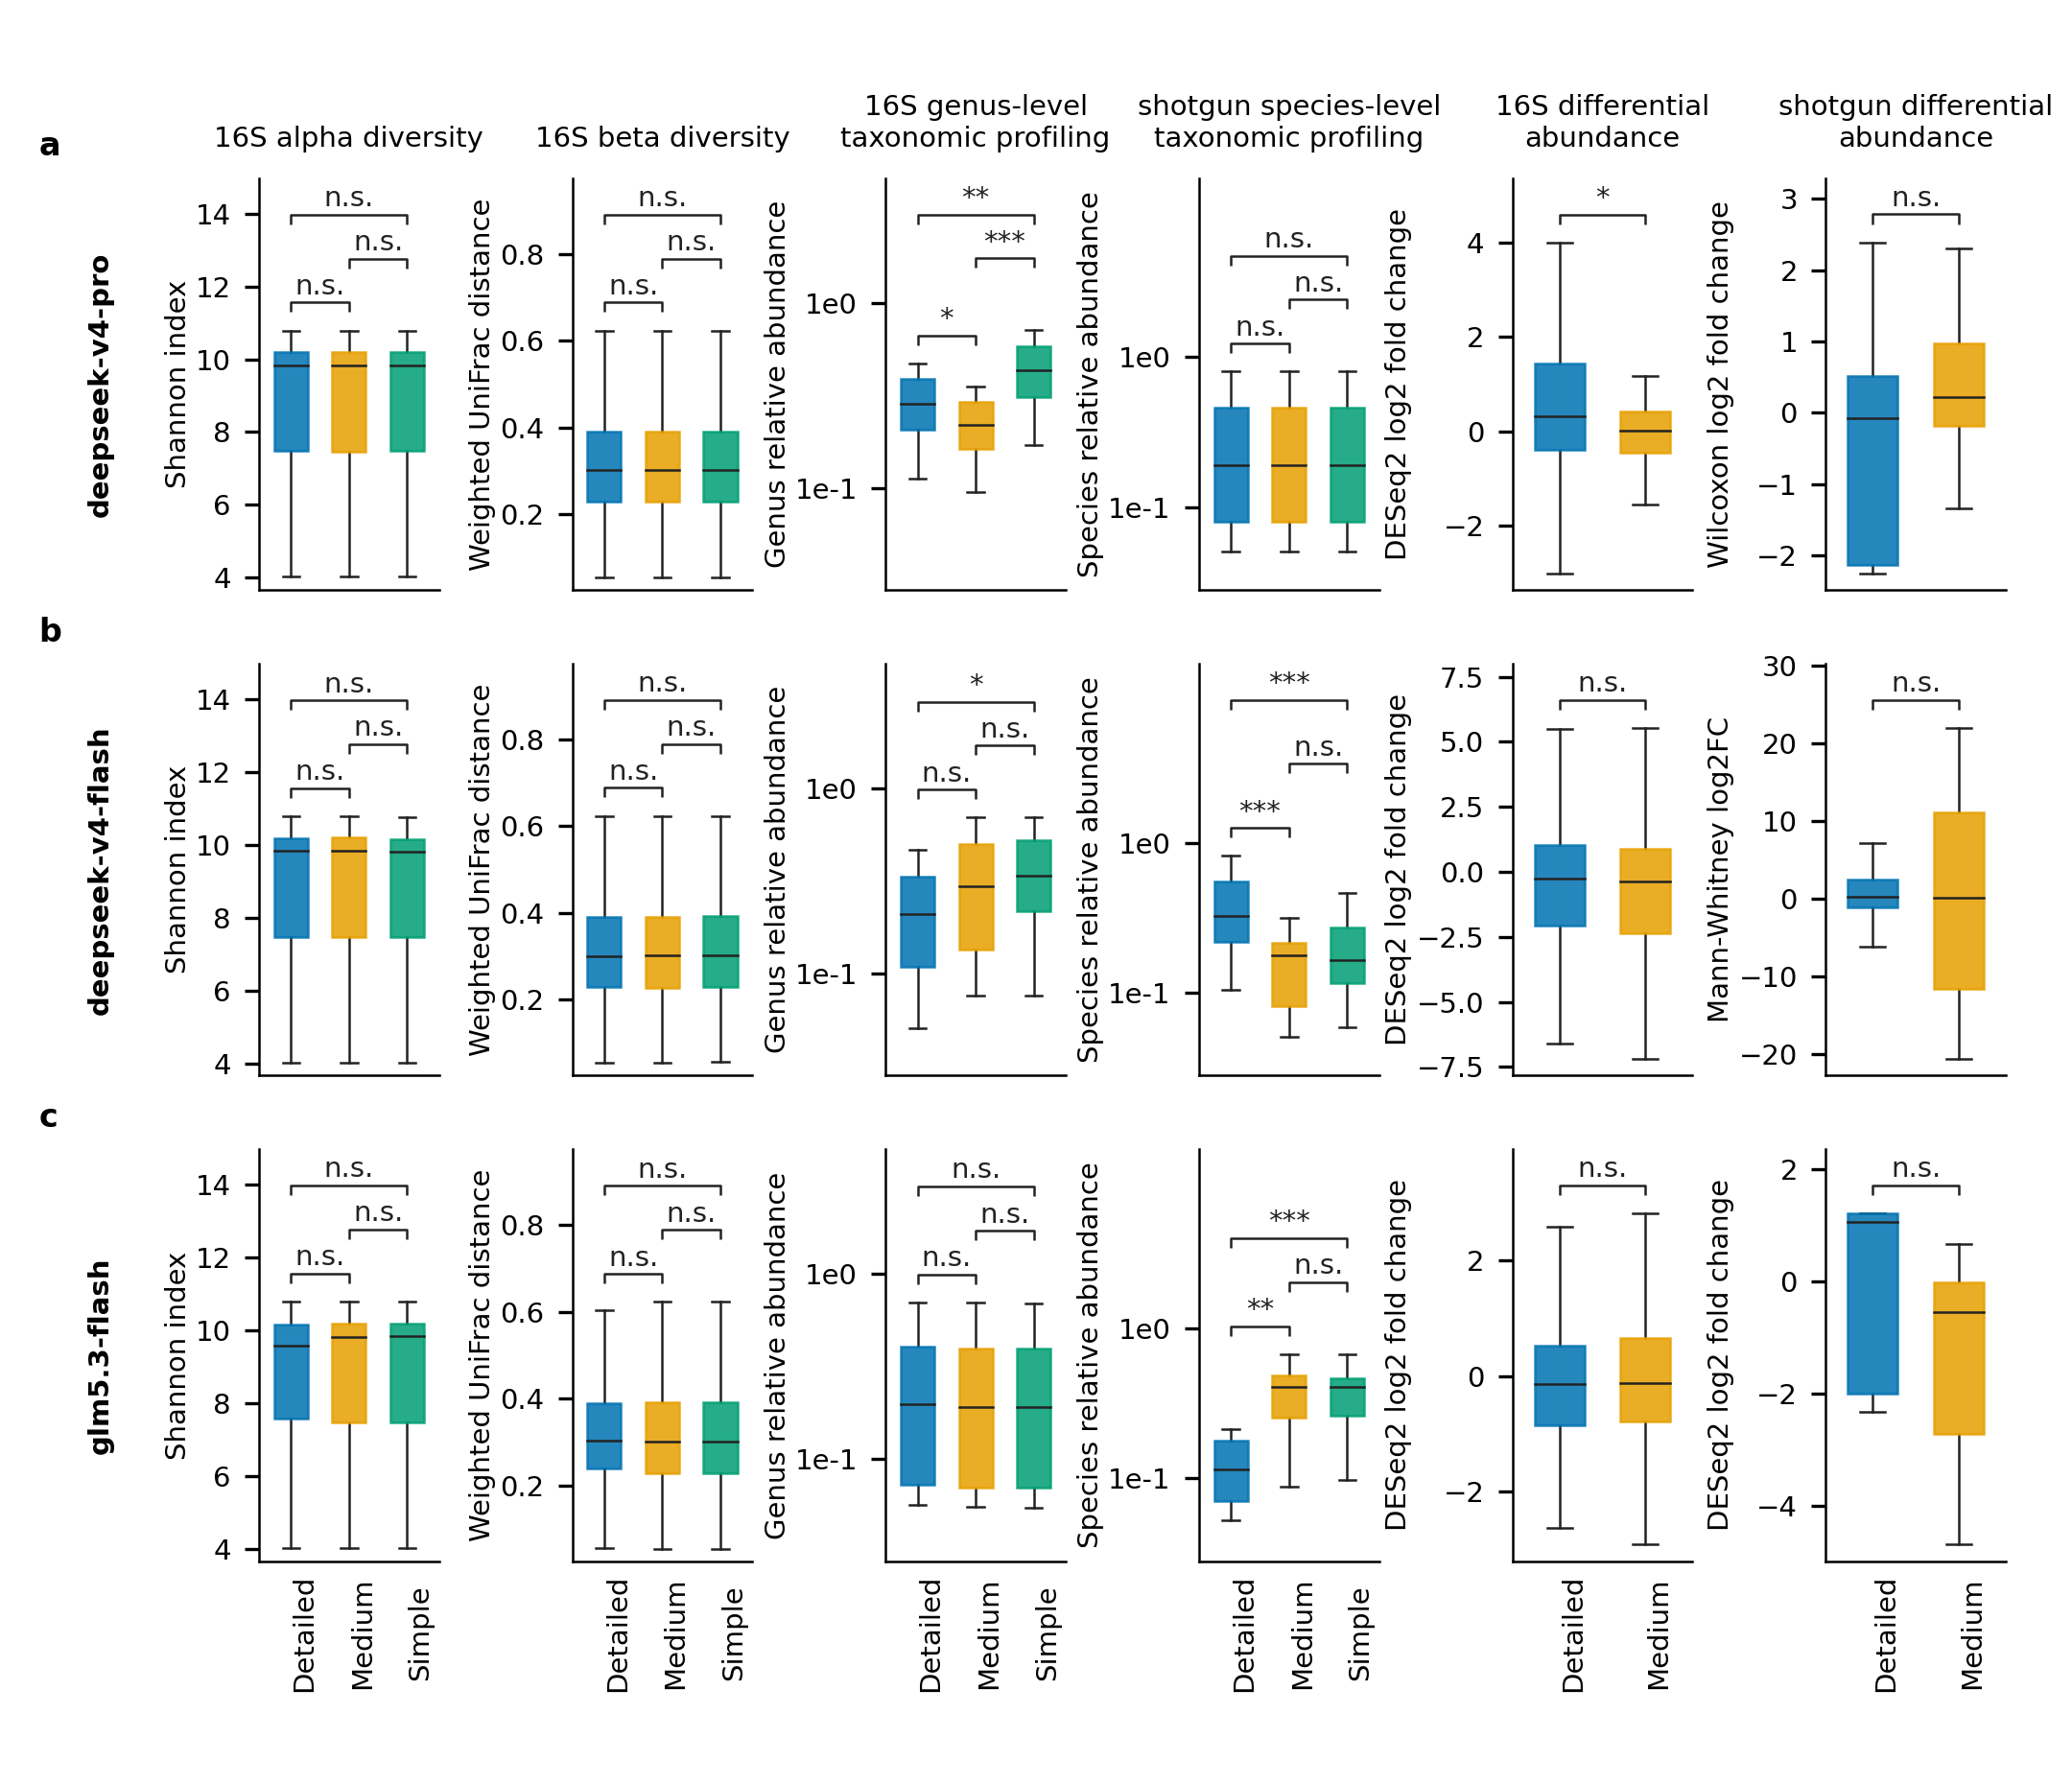
\includegraphics[width=0.92\linewidth]{by_prompt_models.png}
\caption{Comparison of analytical outputs across prompt levels within each
  model. Rows represent \texttt{deepseek-v4-pro}, \texttt{deepseek-v4-flash},
  and \texttt{glm5.3-flash}. The first four columns display 16S Shannon
  diversity indices, pairwise weighted UniFrac distances, 16S genus-level
  relative abundances, and shotgun species-level relative abundances across
  prompt levels. The remaining two columns compare differential-abundance
  $\log_2$ fold changes between the detailed and medium prompts (16S: DESeq2;
  shotgun: the test shared within each model,
  Table~\ref{tab:da-prompt-methods}). Brackets in the first four columns
  indicate two-sided Mann--Whitney $U$ tests with Holm correction across the
  three prompt pairs within each model; brackets in the differential-abundance
  panels indicate comparisons between the detailed and medium prompts. *$P <
  0.05$; **$P < 0.01$; ***$P < 0.001$; n.s., adjusted $P \ge 0.05$. Values are
  derived from repeated analyses of the same Case~1 dataset and do not represent
  independent biological replicates.}
\label{fig:robustness-prompts}
\end{figure}

% Keep the ablation description and its table on the same page.
\clearpage
Table~\ref{tab:ablation-replicates} provides per-session outputs, method
adherence, model and tool calls, and token consumption for the execution
ablation.

\begin{table}[H]
\centering
\caption{Per-session outputs, method adherence, tool calls, and token
  consumption in the execution ablation.}
\label{tab:ablation-replicates}
\normalsize
\setlength{\tabcolsep}{4pt}
\renewcommand{\arraystretch}{1.12}
\textbf{(a) Outputs, method adherence, and model calls}\par\smallskip
\begin{tabular*}{\linewidth}{@{\extracolsep{\fill}}llccc@{}}
\toprule
Condition & Session
  & \shortstack{Outputs\\(of 9)}
  & \shortstack{Methods\\(of 8)}
  & \shortstack{Model\\calls} \\
\midrule
\texttt{full} & 1 & 9/9 & 8/8 & 150 \\
\texttt{full} & 2 & 9/9 & 8/8 & 124 \\
\texttt{full} & 3 & 9/9 & 8/8 & 126 \\
\texttt{full} & Mean / sum & 27/27 & 24/24 & 133.3 \\
\addlinespace
\texttt{no-patch} & 1 & 8/9 & 8/8 & 211 \\
\texttt{no-patch} & 2 & 9/9 & 8/8 & 403 \\
\texttt{no-patch} & 3 & 9/9 & 8/8 & 245 \\
\texttt{no-patch} & Mean / sum & 26/27 & 24/24 & 286.3 \\
\bottomrule
\end{tabular*}
\par\medskip
\textbf{(b) Tool calls and token consumption}\par\smallskip
\begin{tabular*}{\linewidth}{@{\extracolsep{\fill}}llcccc@{}}
\toprule
Condition & Session
  & \texttt{exec}
  & \shortstack{\texttt{process}}
  & \shortstack{\texttt{yield}}
  & \shortstack{Tokens\\($\times 10^6$)} \\
\midrule
\texttt{full} & 1 & 91 & 1 & 17 & 12.92 \\
\texttt{full} & 2 & 74 & 21 & 5 & 14.81 \\
\texttt{full} & 3 & 82 & 0 & 13 & 15.84 \\
\texttt{full} & Mean / sum & 82.3 & 7.3 & 11.7 & 14.53 \\
\addlinespace
\texttt{no-patch} & 1 & 77 & 102 & 0 & 23.77 \\
\texttt{no-patch} & 2 & 142 & 227 & 0 & 49.32 \\
\texttt{no-patch} & 3 & 99 & 136 & 0 & 32.15 \\
\texttt{no-patch} & Mean / sum & 106.0 & 155.0 & 0.0 & 35.08 \\
\bottomrule
\end{tabular*}
\par\vspace{0.4em}
{\normalsize Summary rows pool outputs and method requirements across the three
  sessions. Tool-call counts and token consumption in those rows are per-session
  means. Total tokens are input plus output tokens, including reasoning tokens.}
\end{table}

\end{document}
